\chapter{Results}\label{chp:results}
This chapter will discuss the results obtained during the development of this PhD project.
As described in the previous chapter, a cascade of three modelling tools were employed: a climate model (RegCM, \cref{sec:regcm}), a hydrological model (CHyM, \cref{sec:chym}) and a hydraulic model (CA2D, \cref{sec:ca2d}).
The three models were applied in sequence, with the hydrological model utilising rainfall from the RCM, and the hydraulic model taking as input the discharge data processed with the procedure described in \cref{sec:3_mod_apprach}.

In the following, the RegCM simulations driven by ERA-Interim and HadGEM will be referred to as RegCM-ERA and RegCM-HAD respectively.
Similarly, the CHyM simulations driven by RegCM-ERA and RegCM-HAD are called CHyM-ERA and CHyM-HAD, while the simulation driven by GRIPHO is referred to as CHyM-OBS.
The four climatological seasons displayed are defined as DJF, MAM, JJA and SON, which refers to the initials of their respective months; in the following, they are referred as winter, spring, summer and autumn.
Whenever possible, the analysis was split by four macroregions with different climatic characteristics: North, Centre, South and Islands. These macroregions are identical to those used in the validation of the GRIPHO dataset (\cref{sec:valid_itaobs}).

Five different timeslices are used through this analysis:
\begin{description}
    \item[2001--2016] Validation period for CHyM-OBS.
    \item[1980--2016] Validation period for RegCM-ERA and CHyM-ERA.
    \item[1976--2005] Validation period for RegCM-HAD and CHyM-HAD. This period is also used as reference period for change assessment against the future scenario and is referred to as \emph{historical} or \emph{reference}.
    \item[2020--2049] First time slice for the future scenario simulated by RegCM-GEM and CHyM-HAD. Referred to as \emph{near future}.
    \item[2070--2099] Second time slice for the future scenario simulated by RegCM-HAD and CHyM-HAD. Referred to as \emph{far future} or \emph{end of century}.
\end{description}

The chapter is organised as follows.
In \cref{sec:results_regcm} the validation and future change of mean and extreme precipitation in the RegCM simulations will be presented and discussed.
\Cref{sec:results_chym} will describe the results from the hydrological simulations for both the present day and for the future scenario, including several proxies for future changes in flood hazard.
\Cref{sec:results_flood} will present the preliminary results obtained in creating flood hazard maps for the entire Italian territory, together with a case study regarding a flooding event in north-western Italy.

\section{Validation and future changes of precipitation in the RegCM simulations}\label{sec:results_regcm}
The two climate simulations described in \cref{sec:experiments} are here analysed with particular attention towards extreme precipitation events.
The same precipitation metrics described in \cref{sec:valid_itaobs} are employed.
They are: annual cycle, mean seasonal precipitation, extreme seasonal precipitation ($\textrm{R95}_{ptot}$ and $\textrm{R99}_{ptot}$) and daily precipitation distribution (Probability Density Functions).
Both a present day evaluation and an assessment of future changes (only for the HadGEM-driven simulation) are carried out.
When calculating $\textrm{R95}_{ptot}$ and $\textrm{R99}_{ptot}$ metrics for the future scenario, the 95th and 99th percentile thresholds of the reference period have been used, to provide a uniform reference value.

%------------------------------------
%	PR VALIDATION
%------------------------------------
\subsection{Validation of present-day model performance}\label{sec:valid_regcm}
\Cref{fig:valid_rcm_pr_ac} shows the annual cycle of precipitation over the four macroregions. the performance of the models in reproducing the precipitation annual cycle and the seasonal precipitation respectively, compared against the best available precipitation datasets (see \cref{sec:uncertainty_pr,sec:valid_itaobs} for a comparison of observations).
The annual cycle is approximately correct in the models, with a underestimation (overestimation) of average precipitation occurs in both simulations in the North in autumn (spring).
In particular, the RegCM-ERA simulation is capable of reproducing the November precipitation peak in the Centre, South and Islands.

\Cref{fig:valid_rcm_pr_mean} Average precipitation peaks over the Alps are correctly reproduced, although the models show a tendency to create isolated precipitation hot-spots.
Autumn and winter  precipitations over the west coast of Central and Southern Italy (present in GRIPHO, but not in E-OBS) are correctly reproduced, while an underestimation is present in winter over Liguria and the Gulf of Genoa; an underestimation in the Po plain in winter is present, compared to all the observational datasets. %TODO should expand on this
Overall, the performance of the two RegCM simulations with mean precipitation metrics is good.
The climatologies of the two RegCM simulations are very similar, indicating that a stable equilibrium is reached and that the model is able to create its own climatic features, independently of the driving data.
This gives us confidence in using the RegCM model in future climate projections.\\
\begin{figure}
    \centering
    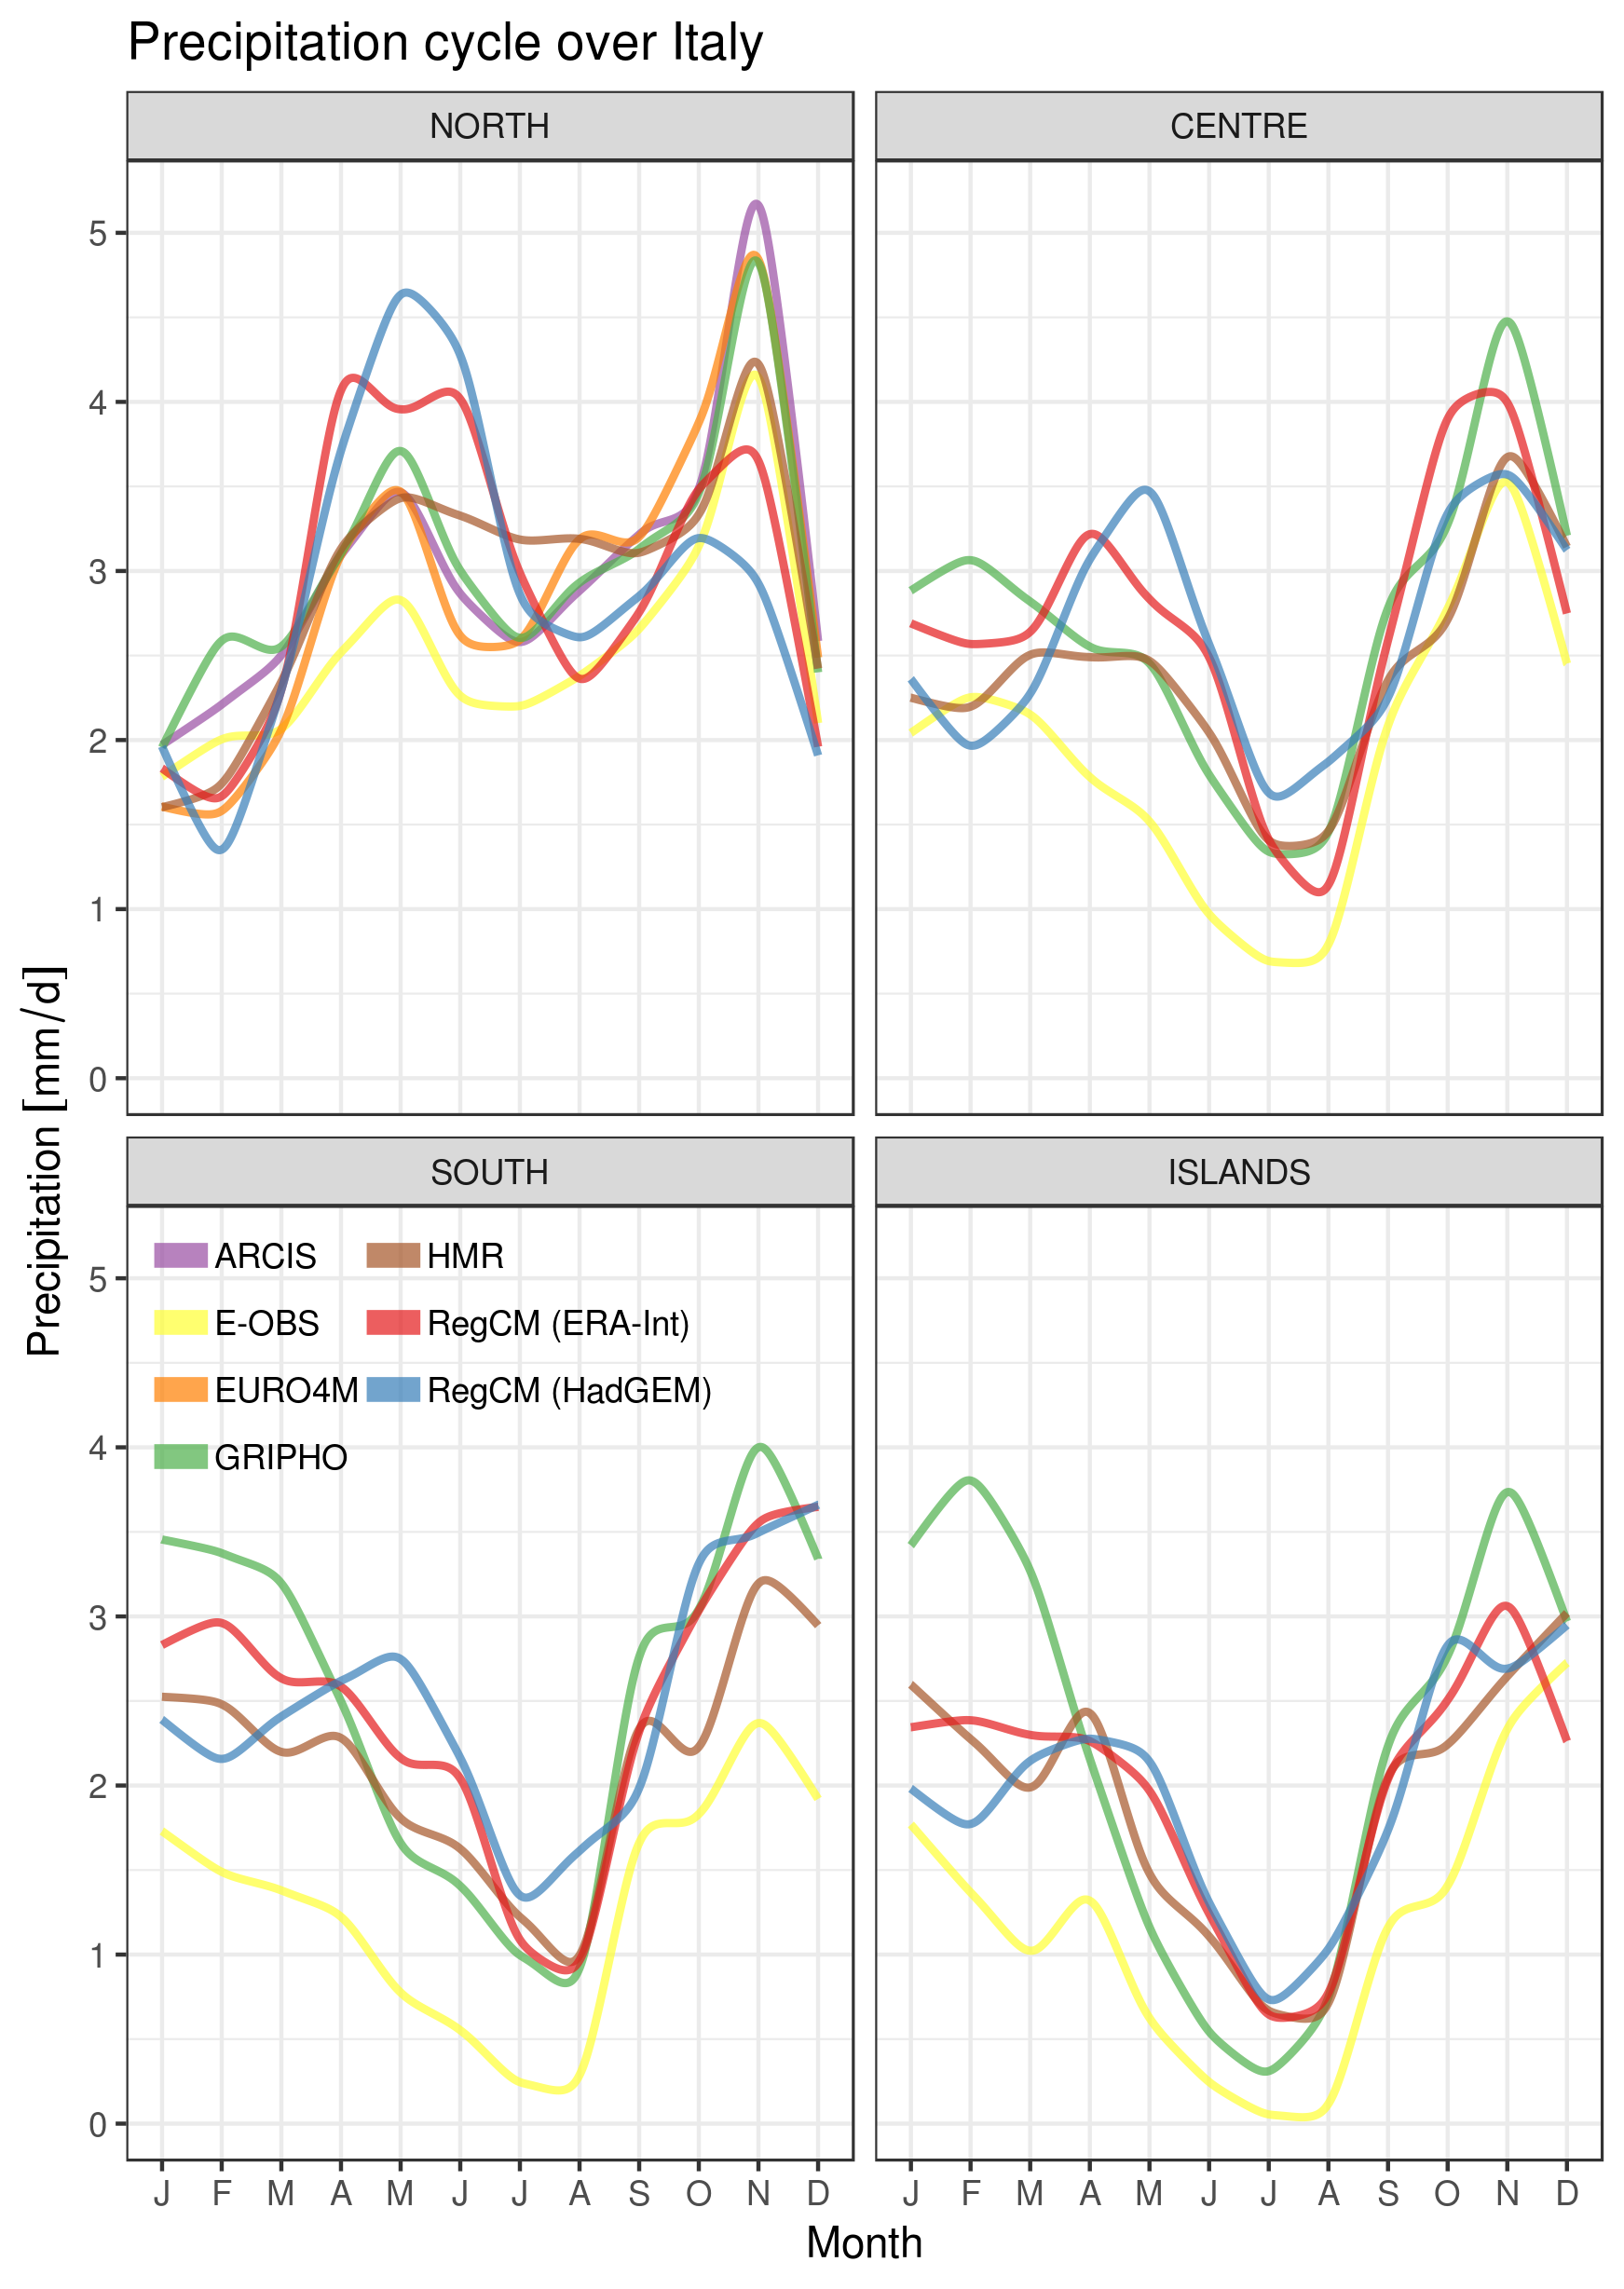
\includegraphics[width=0.7\textwidth]{figures/valid_rcm/pr/ac}
    \decoRule
    \caption[Validation of precipitation annual cycle]{
        Annual cycle of precipitation as reproduced by observations (see \cref{sec:valid_itaobs}) and models (\cref{sec:experiments}). The time period for each dataset varies according to availability. The four macroregions selected are the same as for previous evaluations (\cref{sec:uncertainty_pr,sec:valid_itaobs}).
    }\label{fig:valid_rcm_pr_ac}
\end{figure}
\begin{figure}
    \centering
    \includegraphics[width=0.8\textwidth]{figures/valid_rcm/pr/mean}
    \decoRule
    \caption[Validation of average seasonal precipitation]{
        Average seasonal precipitation for the two climate model simulations (top two rows) and five selected precipitation datasets.
    } \label{fig:valid_rcm_pr_mean}
\end{figure}
Extreme precipitation is assessed via maps of $\textrm{R95}_{ptot}$ (\cref{fig:valid_rcm_pr_r95}) and $\textrm{R99}_{ptot}$ (not shown, but similar to $\textrm{R95}_{ptot}$), where the spatial features are well reproduced.
The models tend to slightly overestimate extreme precipitation hot-spots especially over the Alps and the prealpine areas of North-Eastern Italy, while slightly underestimating in the South when compared to GRIPHO.
Of the two simulations, the ERA-Interim-driven one usually produces more extreme precipitation.
% Given that none of the observational datasets here considered have any kind of undercatch correction, this overestimation is not surprising.
PDFs of daily precipitation (\cref{fig:valid_rcm_pr_pdf1,fig:valid_rcm_pr_pdf2}) for the four regions and seasons generally show a slight underestimation of extremely strong events compared to the GRIPHO gridded dataset presented in \cref{chp:itaobs}, with intermediate values lower than \SI{200}{\milli\metre\per\day} slightly more underestimated.
In the North, the PDFs of the models resemble more closely the high resolution datasets (GRIPHO, ARCIS, EURO4M) than the lower resolution E-OBS.
In Central Italy in summer RegCM-HAD slightly underestimates extreme precipitations compared to GRIPHO, which however is likely affected by erroneous station data for a few grid points in summer over that region (see \cref{sec:valid_itaobs}).
Neither model can reproduce the high precipitations found in winter and spring on the east coast of Sardinia, which both GRIPHO and HMR (but not E-OBS) show.
The extreme precipitation over Mount Etna in Sicily, reported by HMR, is also underestimated.
Comparing RegCM-ERA and RegCM-HAD reveals a difference in the extreme tail of the distribution, where the former generally produces more precipitation extremes (except in summer in the South).
Compared to E-OBS and HMR extremes are systematically overestimated, which is likely due to the low station density of these datasets.
This underlines the necessity of high-resolution datasets with a large number of stations in order to properly validate extreme precipitations.
Similar conclusions were reached before in other studies \citep{Fantini2016,Prein2016,Prein2017}.
\begin{figure}
    \centering
    \includegraphics[width=0.8\textwidth]{figures/valid_rcm/pr/r95ptot}
    \decoRule
    \caption[Validation of extreme events ($\textrm{R95}_{ptot}$)]{
        Seasonal $\textrm{R95}_{ptot}$ maps for the two climate model simulations (top two rows) and five selected precipitation datasets.
    } \label{fig:valid_rcm_pr_r95}
\end{figure}
% \begin{figure}
%     \centering
%     \includegraphics[width=0.8\textwidth]{figures/valid_rcm/pr/r99ptot}
%     \decoRule
%     \caption[Validation of extreme events ($\textrm{R99}_{ptot}$)]{
%         Seasonal $\textrm{R99}_{ptot}$ maps for thetwo climate model simulations (top two rows) and five selected precipitation datasets.
%     } \label{fig:valid_rcm_pr_r99}
% \end{figure}
\afterpage{\clearpage}
\begin{sidewaysfigure}
    \centering
        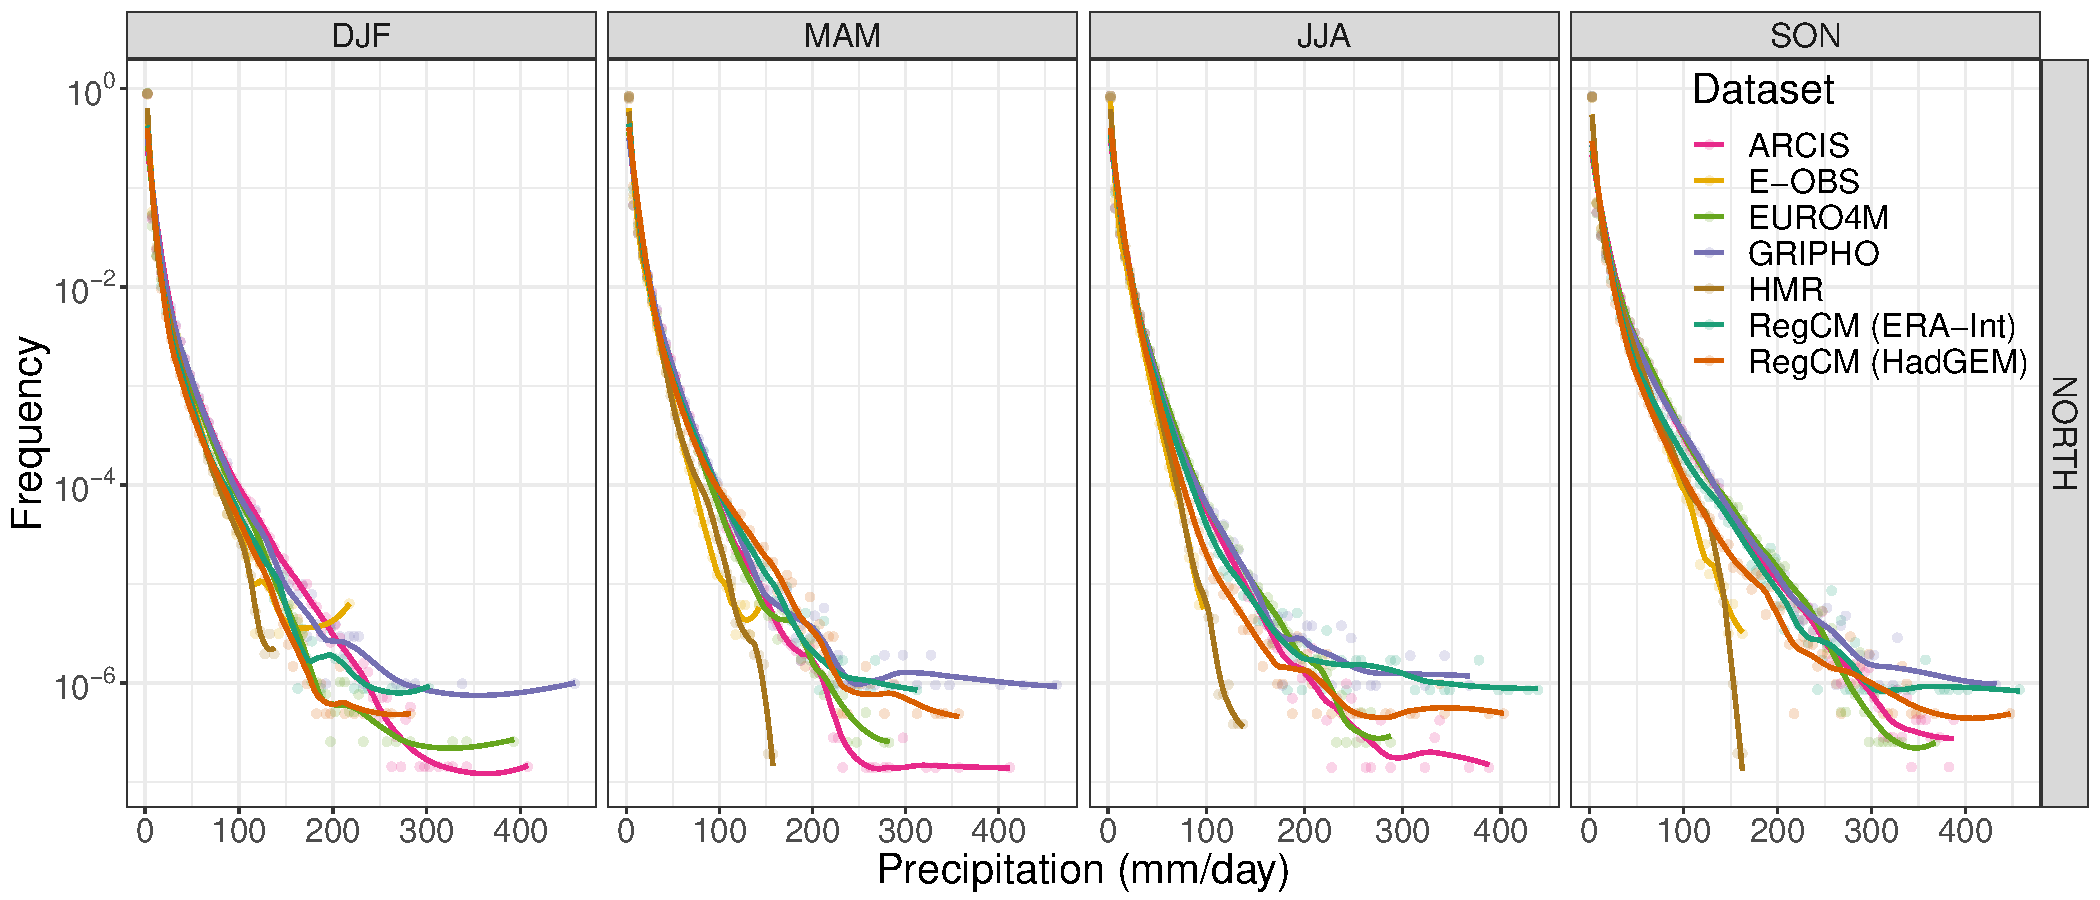
\includegraphics[width=0.8\textheight]{figures/valid_rcm/pr/pdf_NORTH_lines}
        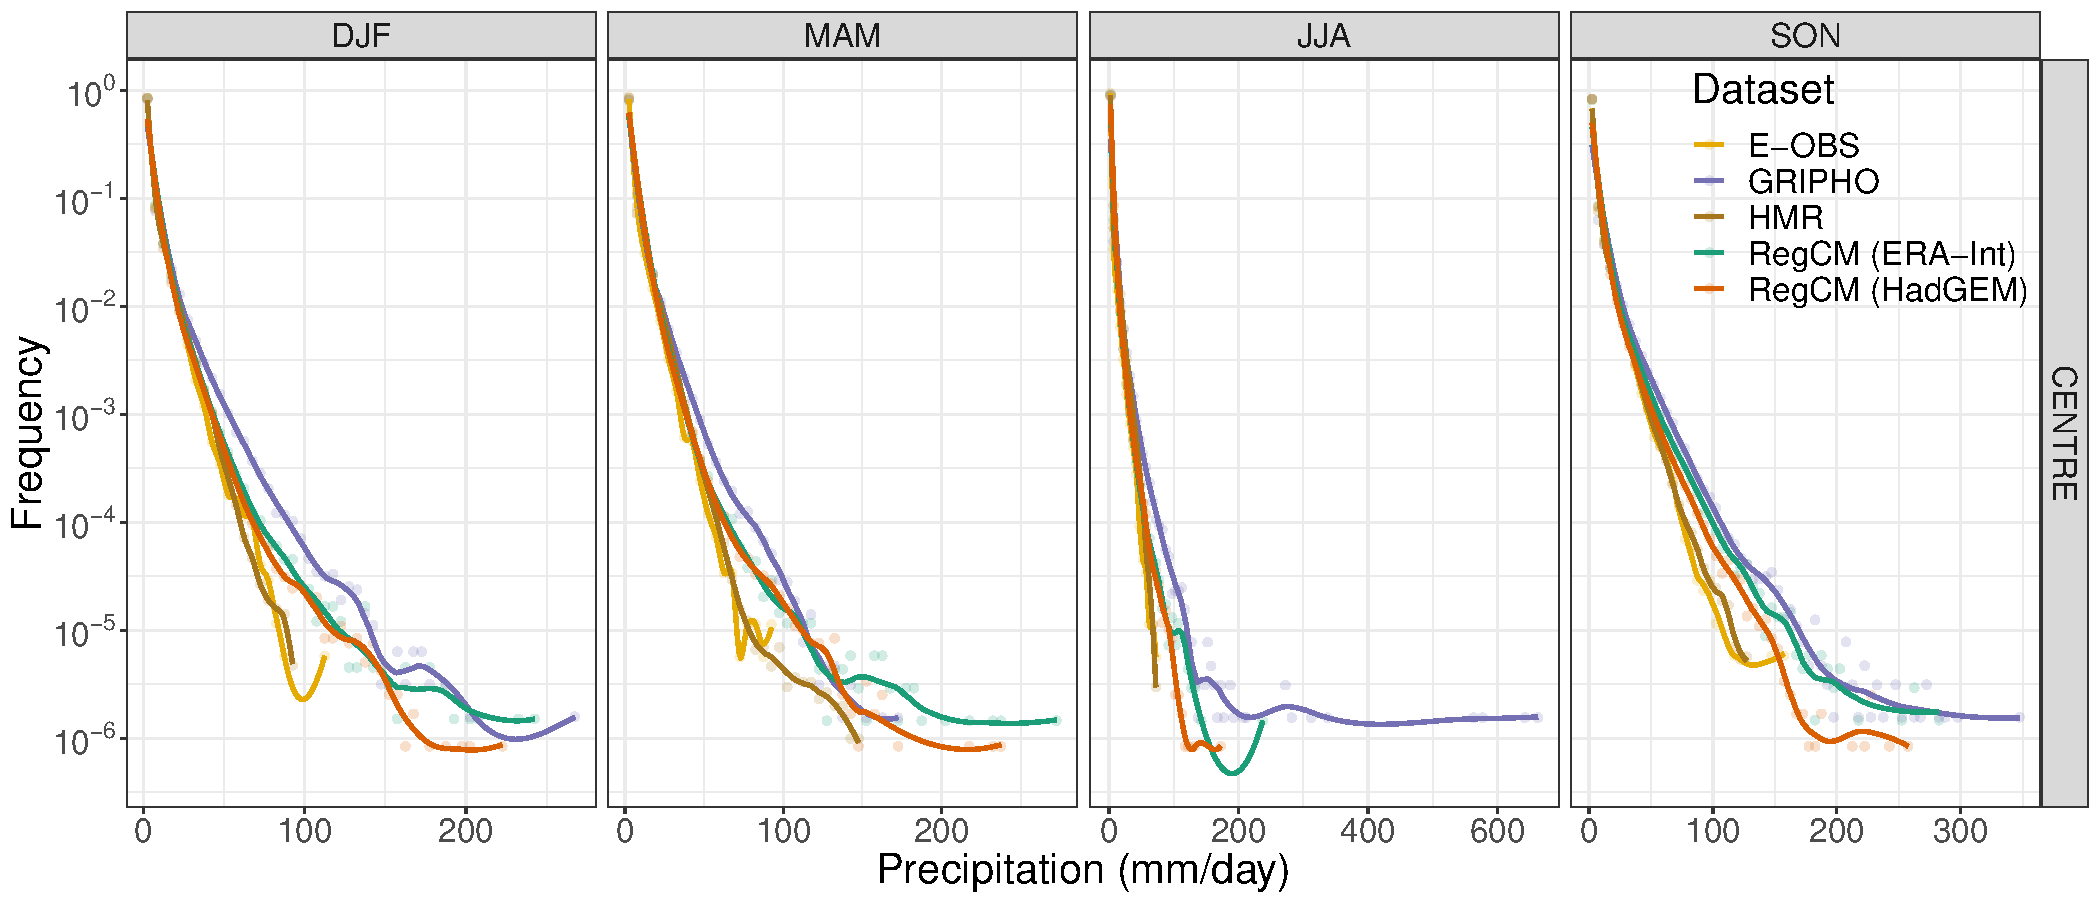
\includegraphics[width=0.8\textheight]{figures/valid_rcm/pr/pdf_CENTRE_lines}
    \caption[Validation of RegCM precipitation PDFs (1)]{
        Daily precipitation Probability Density Functions for the validation of the RegCM simulations for the North and Centre regions. The four summarising regions are highlighted in \cref{fig:valid_rcm_pr_mean,fig:valid_rcm_pr_r95}. The solid lines are smoothed fits.
    }\label{fig:valid_rcm_pr_pdf1}
\end{sidewaysfigure}
\afterpage{\clearpage}
\begin{sidewaysfigure}
    \centering
        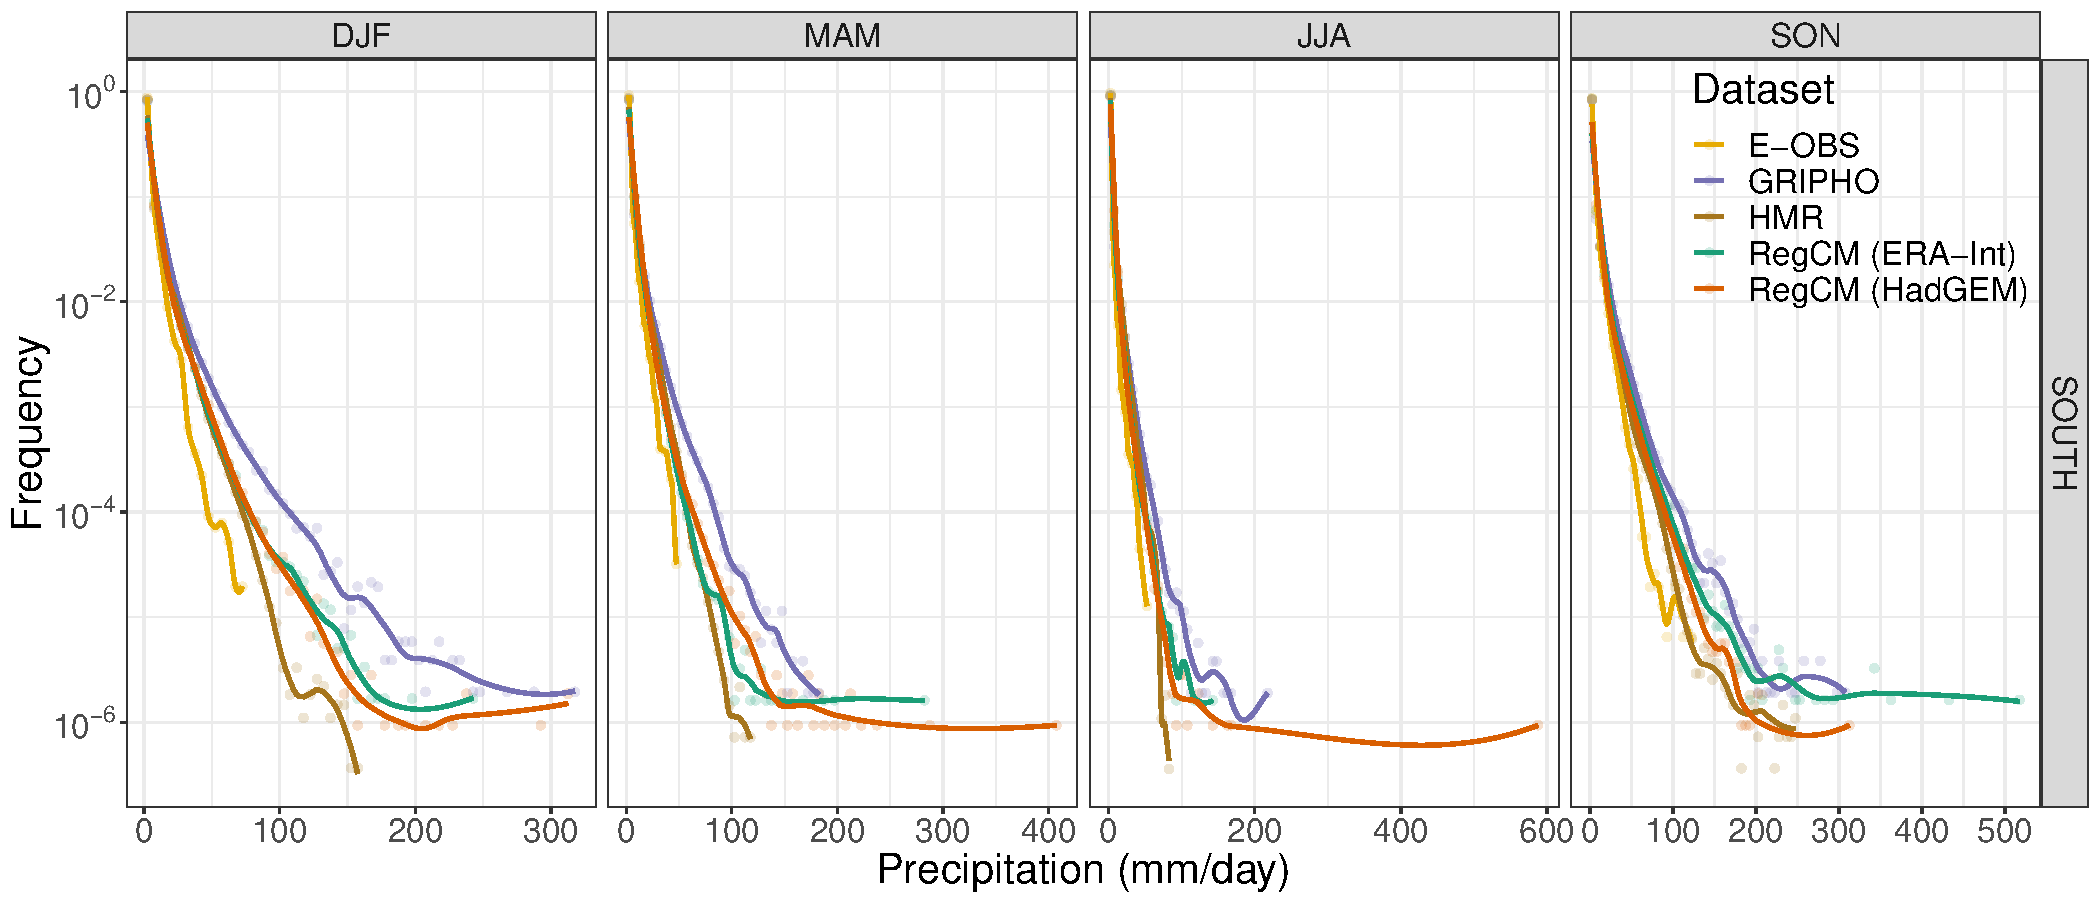
\includegraphics[width=0.8\textheight]{figures/valid_rcm/pr/pdf_SOUTH_lines}
        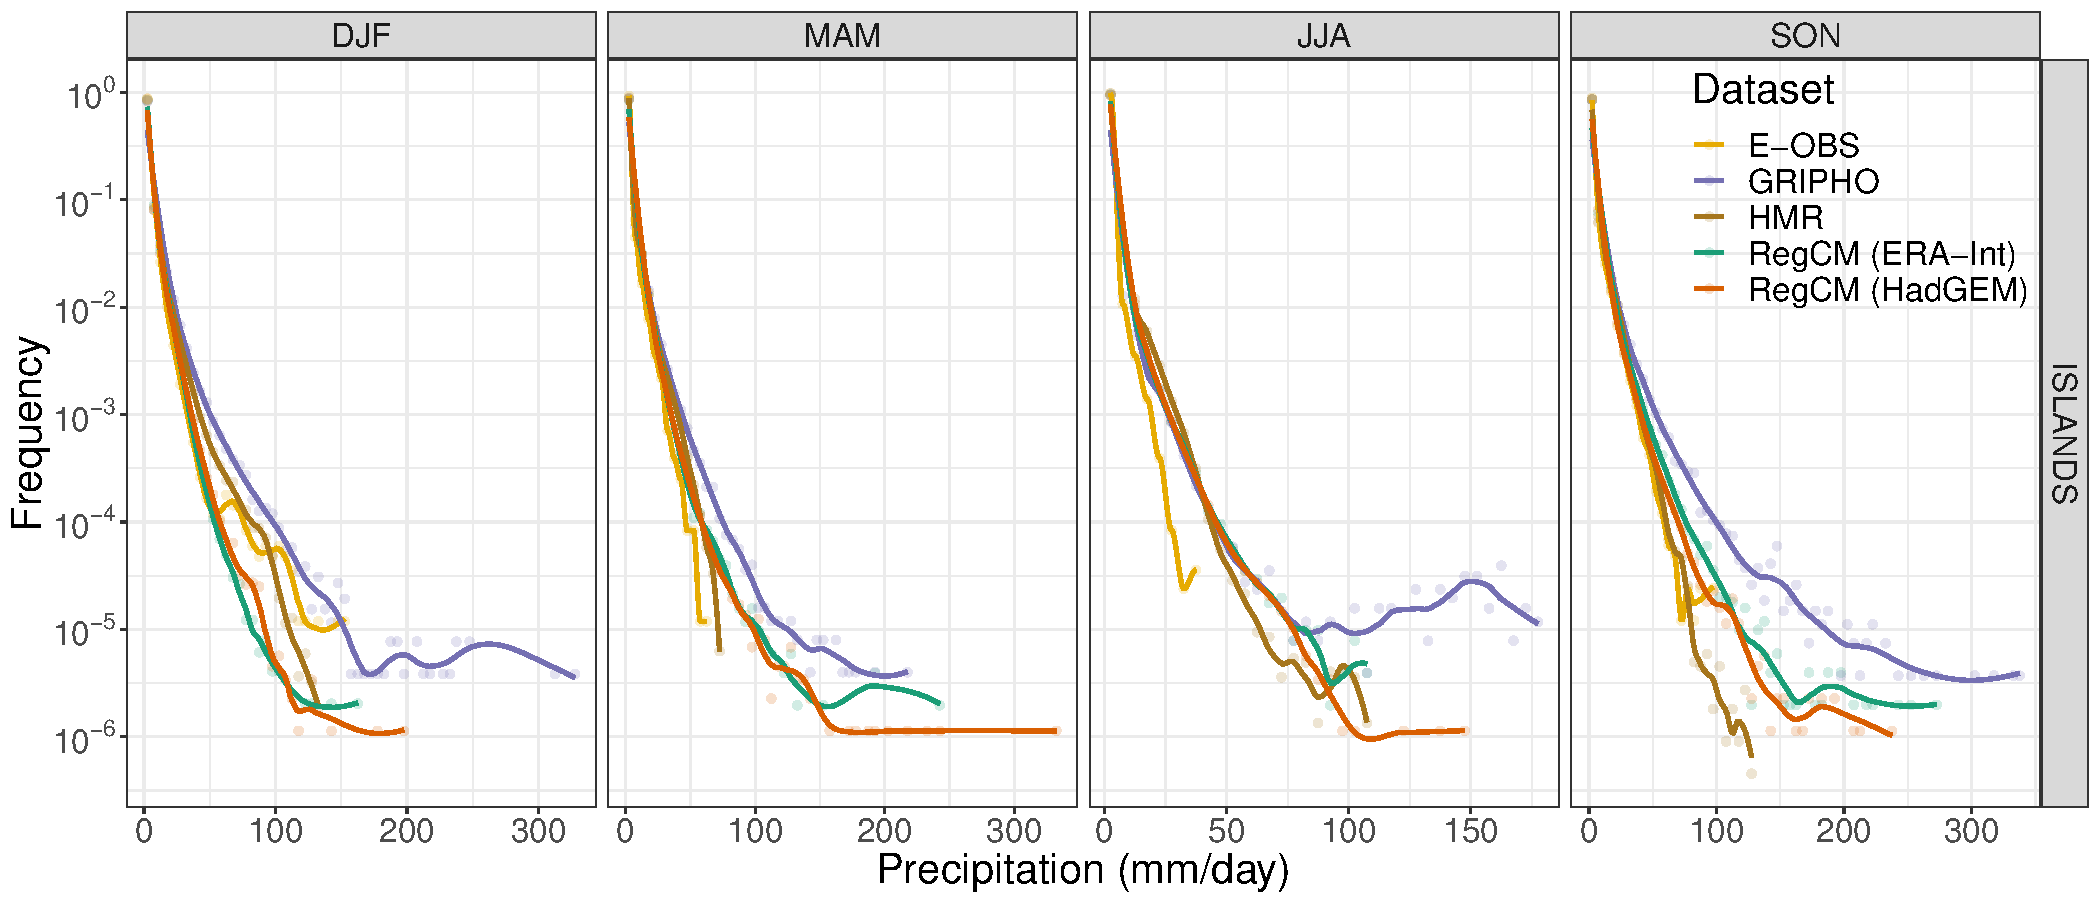
\includegraphics[width=0.8\textheight]{figures/valid_rcm/pr/pdf_ISLANDS_lines}
    \decoRule
    \caption[Validation of RegCM precipitation PDFs (2)]{
        As \cref{fig:valid_rcm_pr_pdf1}, but for the South and Islands regions.
    }\label{fig:valid_rcm_pr_pdf2}
\end{sidewaysfigure}

Evaluation of simulated temperature, which is not as strongly linked to flood events as precipitation, is presented in \cref{appendix_tas}.
Both model simulations show good ability to simulate temperature patterns and averages across the complete study domain.

%------------------------------------
%	PR CHANGE
%------------------------------------
\subsection{Changes in future climate in the RegCM (HadGEM) simulation}\label{sec:change_rcm}
As seen in \cref{sec:future_extremes}, future precipitation is projected to move towards fewer, more extreme precipitation events. We expect this trend to be also highlighted in RegCM-HAD under the RCP8.5 scenario.\\
\Cref{fig:change_rcm_pr_ac} shows the annual cycle of mean precipitation across the three timeslices for RegCM-HAD.
No strong shift in precipitation seasonality, but rather a general decrease of precipitation all year round, except for winter precipitation in the North, which slightly increases.
In the far future, April-May-June precipitation is projected to decrease in all regions but the North
An interesting dual mode of precipitation is produced in the far future in the north, where September precipitation is increased and October precipitation decreases.
Note that the near future average is very close to the reference (1976--2005), due to the nature of the selected RCP, which substantially increases the greenhouse gases forcing only starting from the second half of the century.
Spatial patterns of mean precipitation (\cref{fig:change_rcm_pr_mean}) further highlight the increase in average precipitation in the colder months in the North in both time slices ($+18\%$ for 2020--2049, $+13\%$ for 2070--2099).
A precipitation decrease is instead present in the Islands in all seasons and especially in spring ($-23\%$) and summer ($-31\%$) by the end of the century.
In the other regions, a reduction of summer precipitation can be noted, especially for the far future, with reductions of 14, 13 and $34\%$ for the Centre, South and Islands respectively.
\begin{figure}
    \centering
    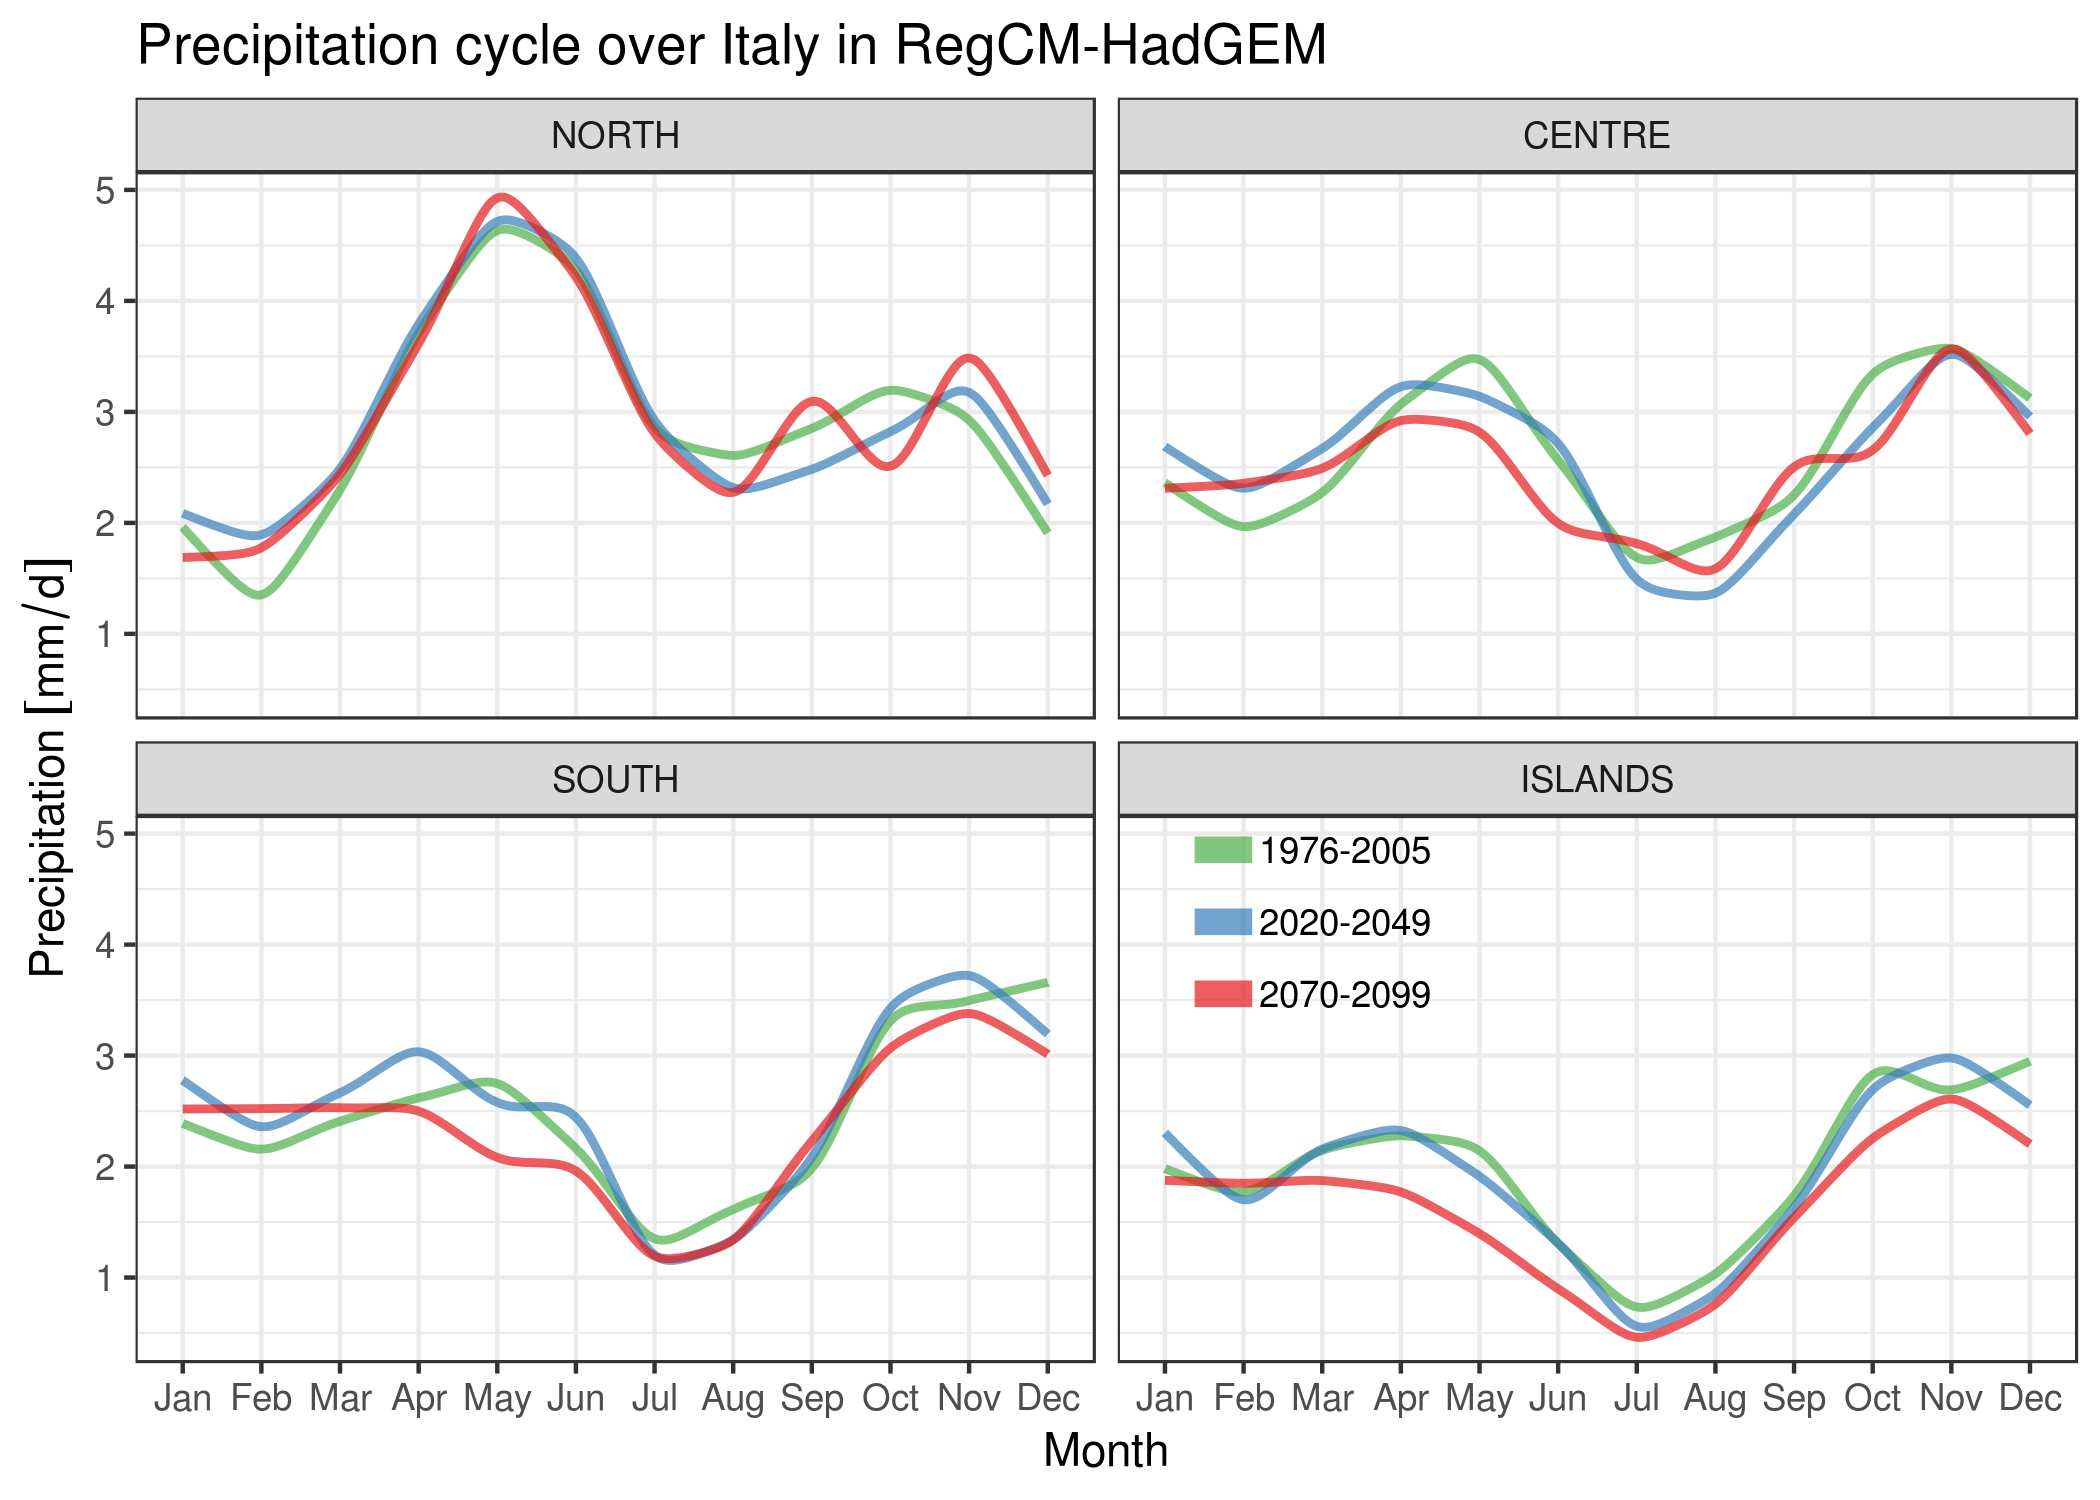
\includegraphics[width=\textwidth]{figures/change_rcm/pr/ac}
    \decoRule
    \caption[Projected change change of the precipitation annual cycle]{
        The precipitation annual cycle for RegCM-HAD in the three timeslices selected, for the four macroregions (see \cref{sec:uncertainty_pr,sec:valid_itaobs}).
    }\label{fig:change_rcm_pr_ac}
\end{figure}
\begin{figure}
    \centering
    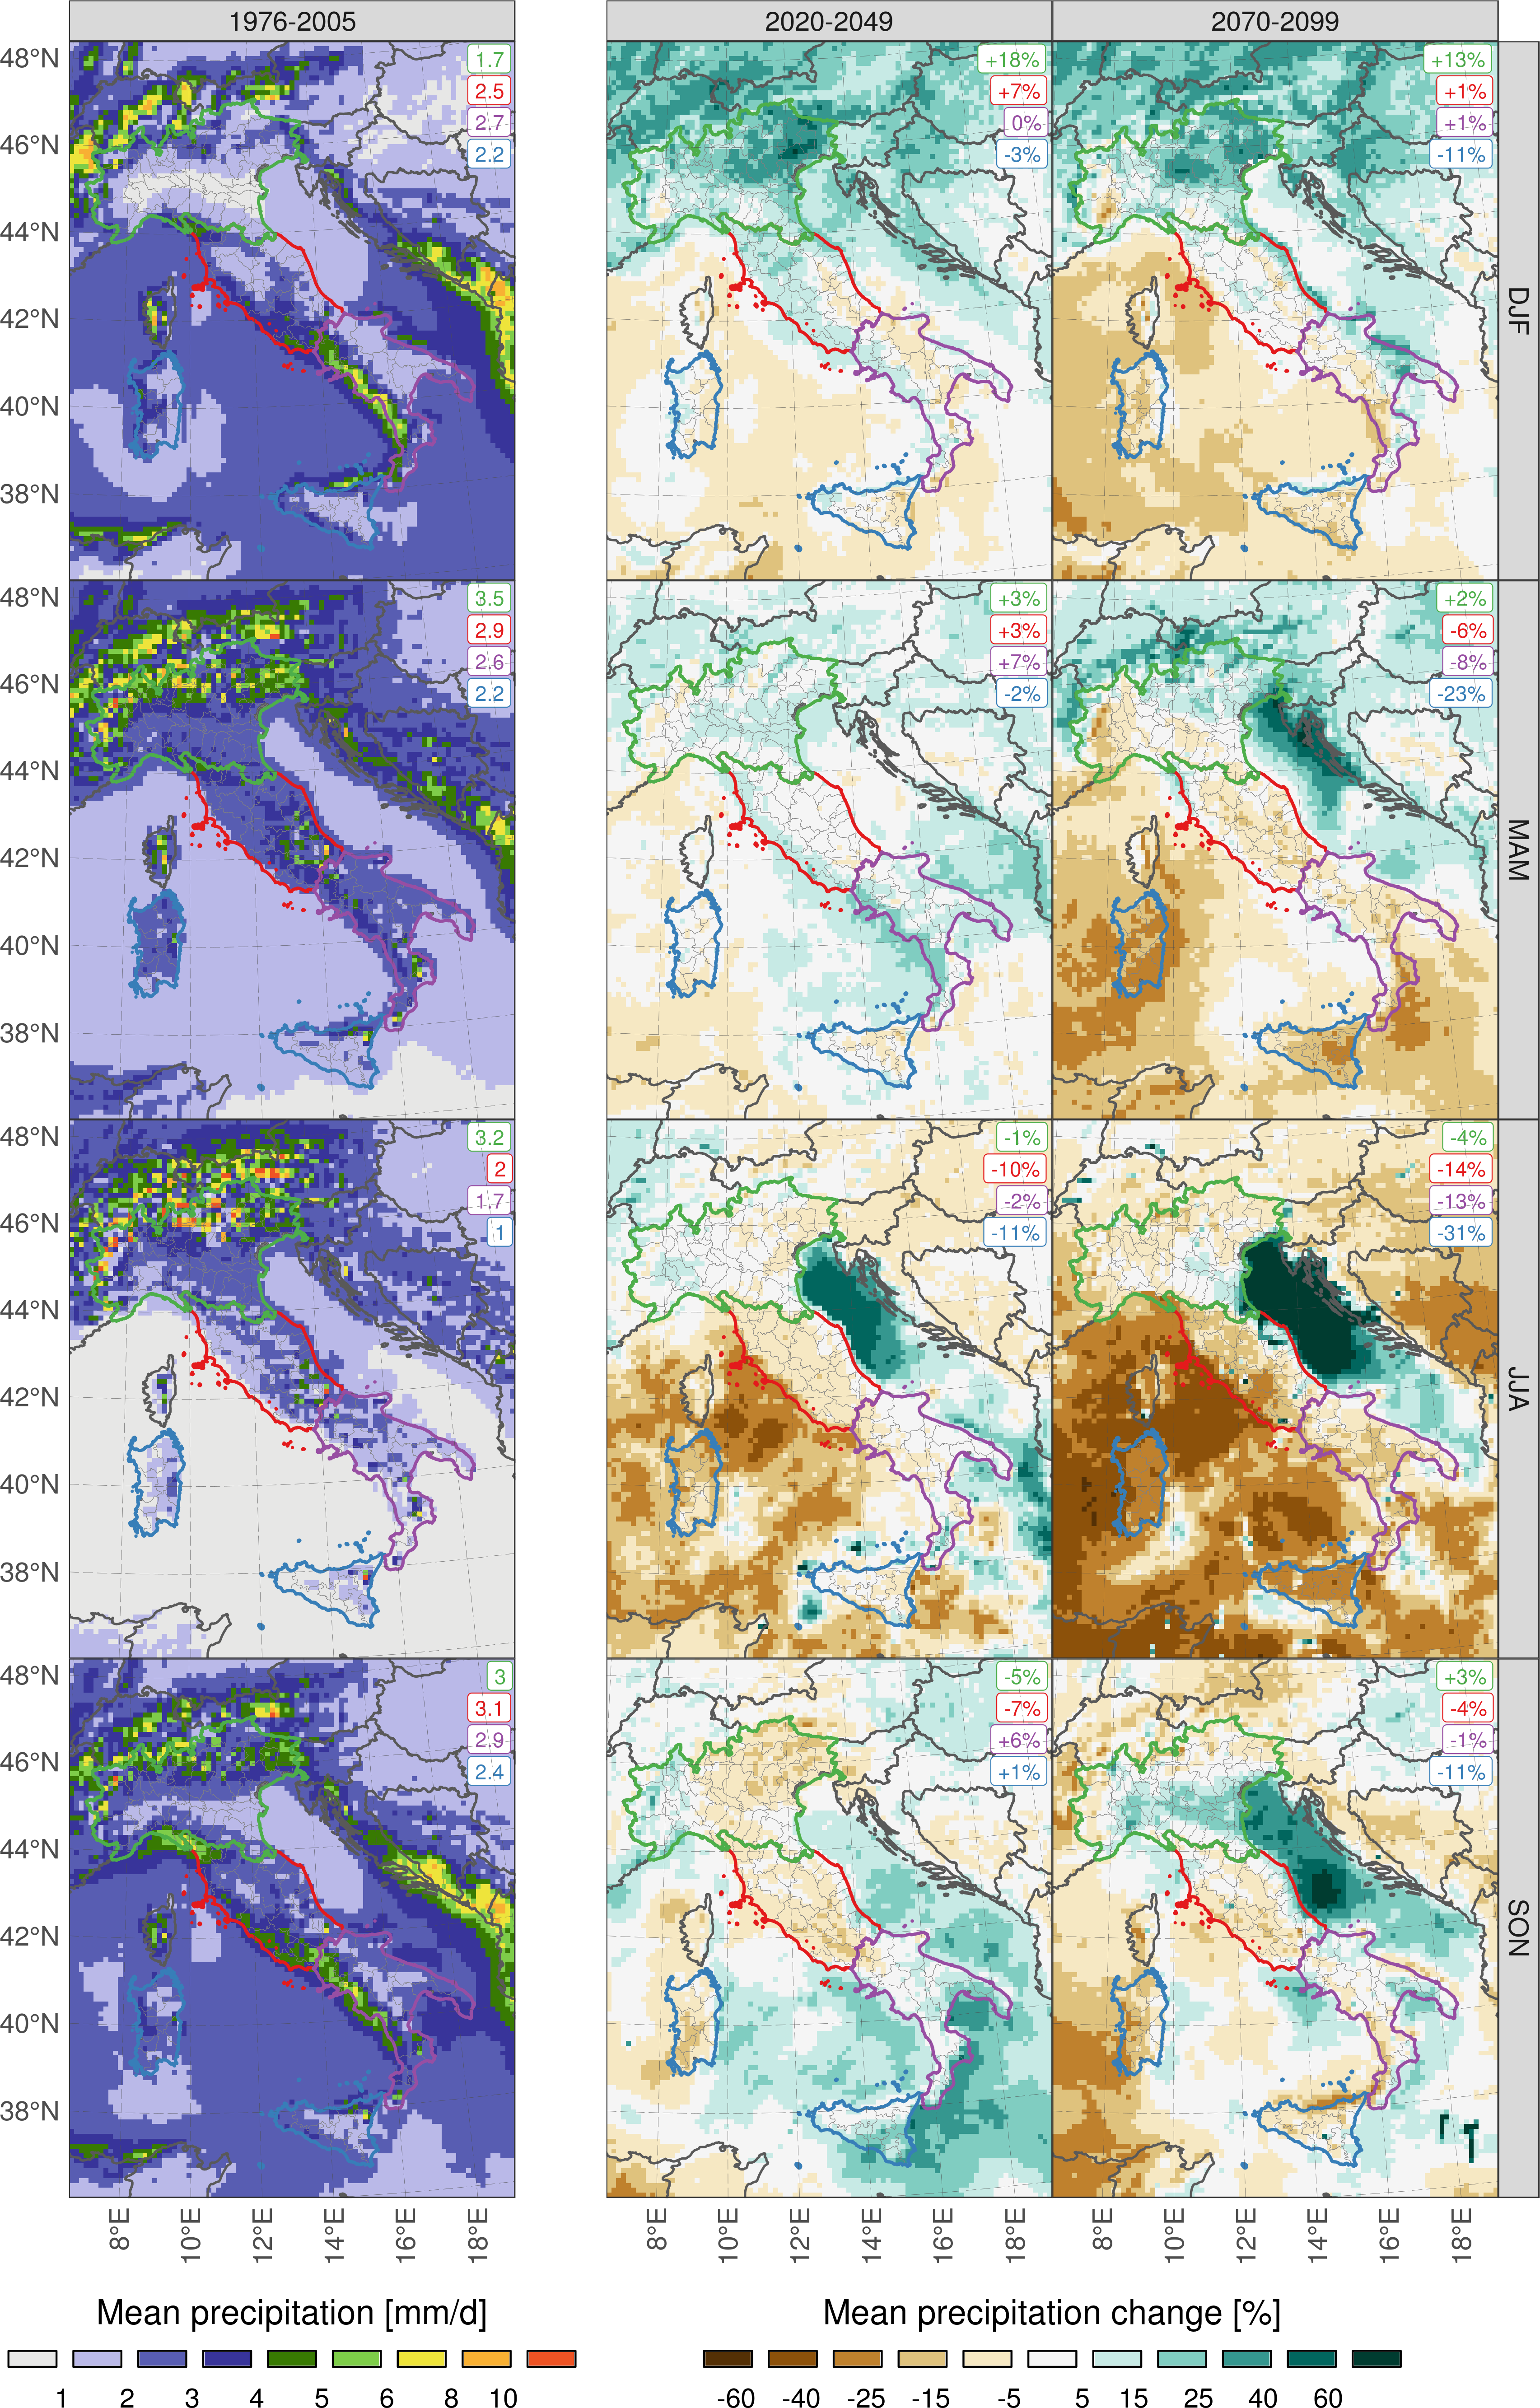
\includegraphics[width=\textwidth]{figures/change_rcm/pr/meanpctl_change_3col}
    \decoRule
    \caption[Projected change of average seasonal precipitation]{
        Average seasonal precipitation for RegCM-HAD for the reference period (left column) and \% change w.r.t. it (centre and right column, in percentage). The four rows represent seasons. In the top right corner of each map, the colour-coded average for each of the four macroregions is shown.
    } \label{fig:change_rcm_pr_mean}
\end{figure}

Changes in precipitation extremes are more relevant for this project. \Cref{fig:change_rcm_pr_r95} shows the evolution across the three timeslices of the extreme $\textrm{R95}_{ptot}$ metric, which is characterised by a general increase in all regions towards the end of the century, with average changes ranging from $+17\%$ to $+58\%$.
For $\textrm{R99}_{ptot}$ (not shown), the changes are even larger and range from $+52\%$ to $+155\%$ in the end of the century period.
Over land, the area that shows the largest signal is the Po plain, especially in winter and autumn, followed by the south-eastern region.
Over high elevations, changes seem to be generally negligible or even slightly negative in all seasons.
Spatial trends across the two future timeslices are similar, but there are nonetheless areas (such as Central Italy in autumn) in which the change signal differs between the two timeslices.
The daily precipitation PDFs (\cref{fig:change_rcm_pr_pdf1,fig:change_rcm_pr_pdf2}) also show a similar increase, with stronger extreme events being more pronounced in the far future and, in several cases, with presence of events of a magnitude not recorded in the historical period.
The changes greatly depend on the region and the season:  Central Italy shows barely any change in winter, but in summer strong events with a magnitude of \SI{100}{\milli\metre\per\day} or greater are ten times more frequent in the far future timeslice than in the reference period.\\
For all regions, autumn shows the largest increase in extreme precipitation, with freater values in Central and Southern Italy
% Once again, the two future timeslices show very different behaviours, with most of the large changes only happening towards the end of the century. % erika mi ha corretto via questo ma non so perché
Overall, the general tendency of increased extreme precipitation is confirmed, even in regions where average precipitation is projected to decrease.
\begin{figure}
    \centering
    \includegraphics[width=\textwidth]{figures/change_rcm/pr/r95_change_3col}
    \decoRule
    \caption[Validation of extreme events ($\textrm{R95}_{ptot}$)]{
        Seasonal $\textrm{R95}_{ptot}$ for RegCM-HAD for the reference period (left column) and \% change w.r.t. it (centre and right column, in percentage). The four rows represent seasons. In the top right corner of each map, the colour-coded average for each of the four macroregions is shown.
    } \label{fig:change_rcm_pr_r95}
\end{figure}
% \begin{figure}
%     \centering
%     \includegraphics[width=0.8\textwidth]{figures/change_rcm/pr/r99_change_3col}
%     \decoRule
%     \caption[Validation of extreme events ($\textrm{R99}_{ptot}$)]{
%         Seasonal $\textrm{R99}_{ptot}$  for RegCM-HAD for the reference period (left column) and \% change w.r.t. it (centre and right column, in percentage). The four rows represent seasons. In the top right corner of each map, the colour-coded average for each of the four macroregions is shown.
%     } \label{fig:change_rcm_pr_r99}
% \end{figure}
\afterpage{\clearpage}
\begin{sidewaysfigure}
    \centering
        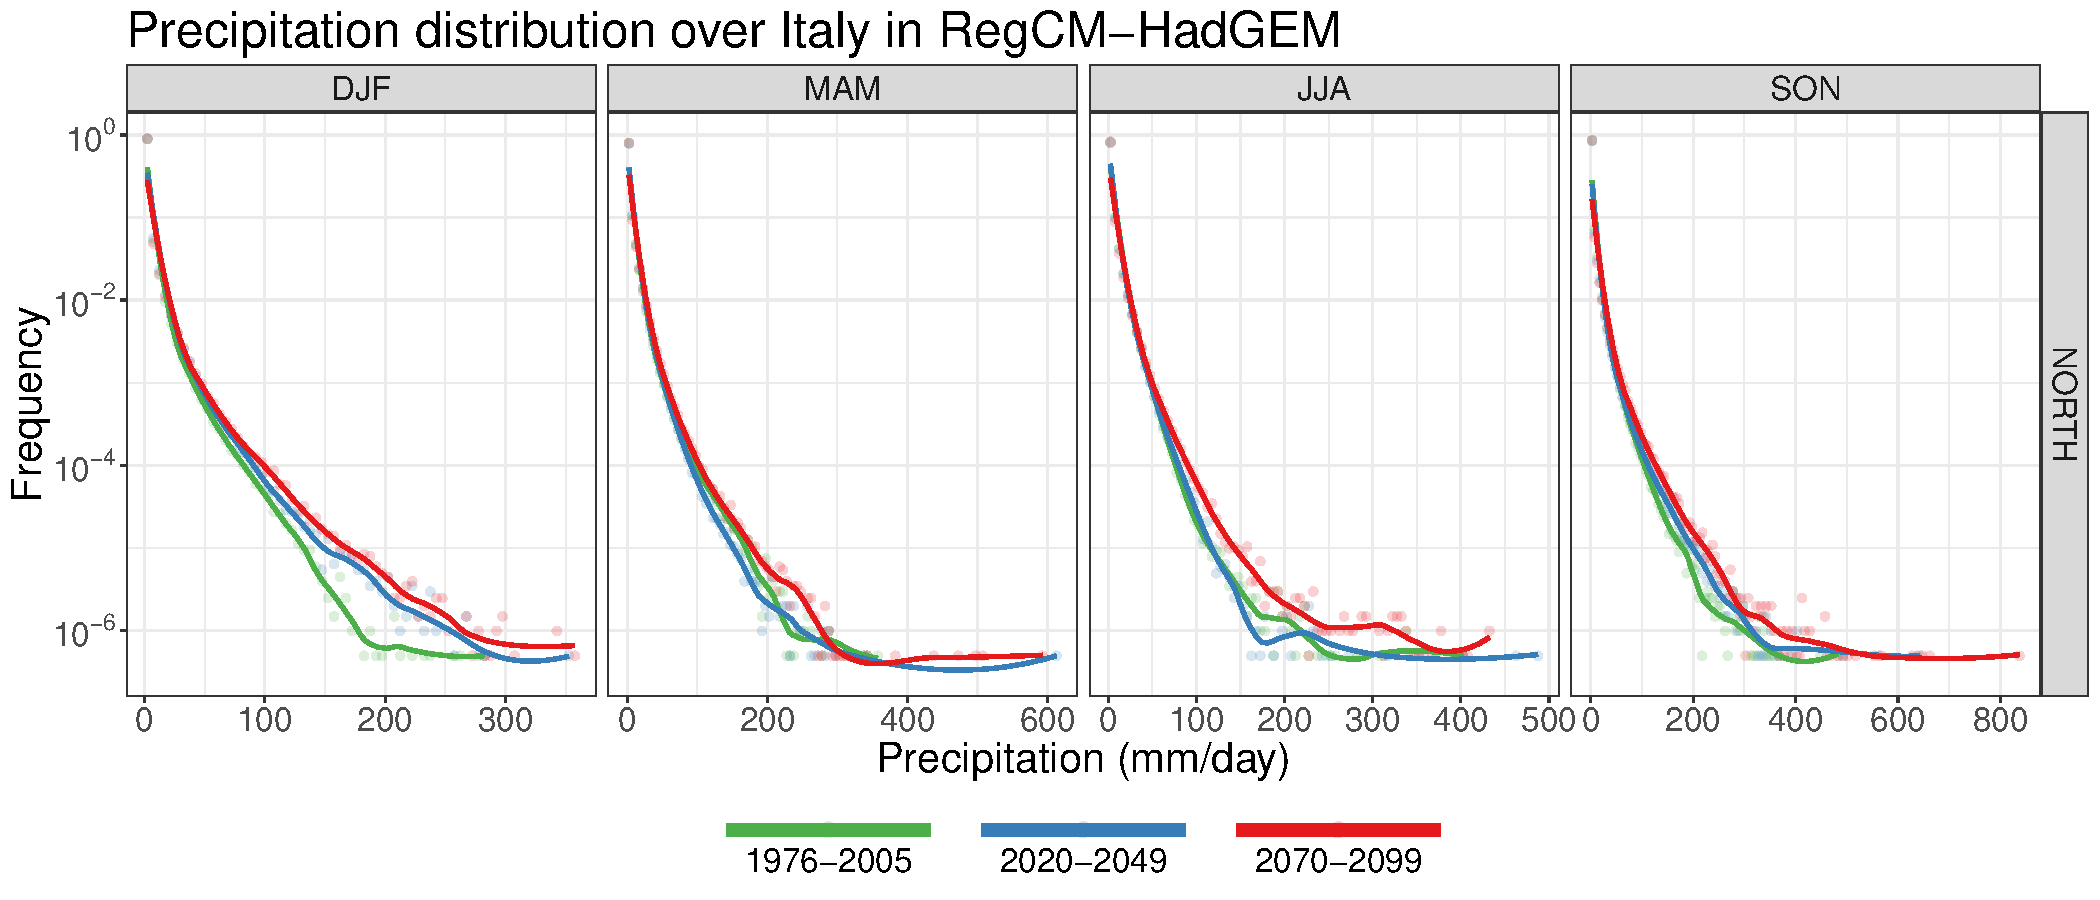
\includegraphics[width=0.8\textheight]{figures/change_rcm/pr/pdf_NORTH_lines}
        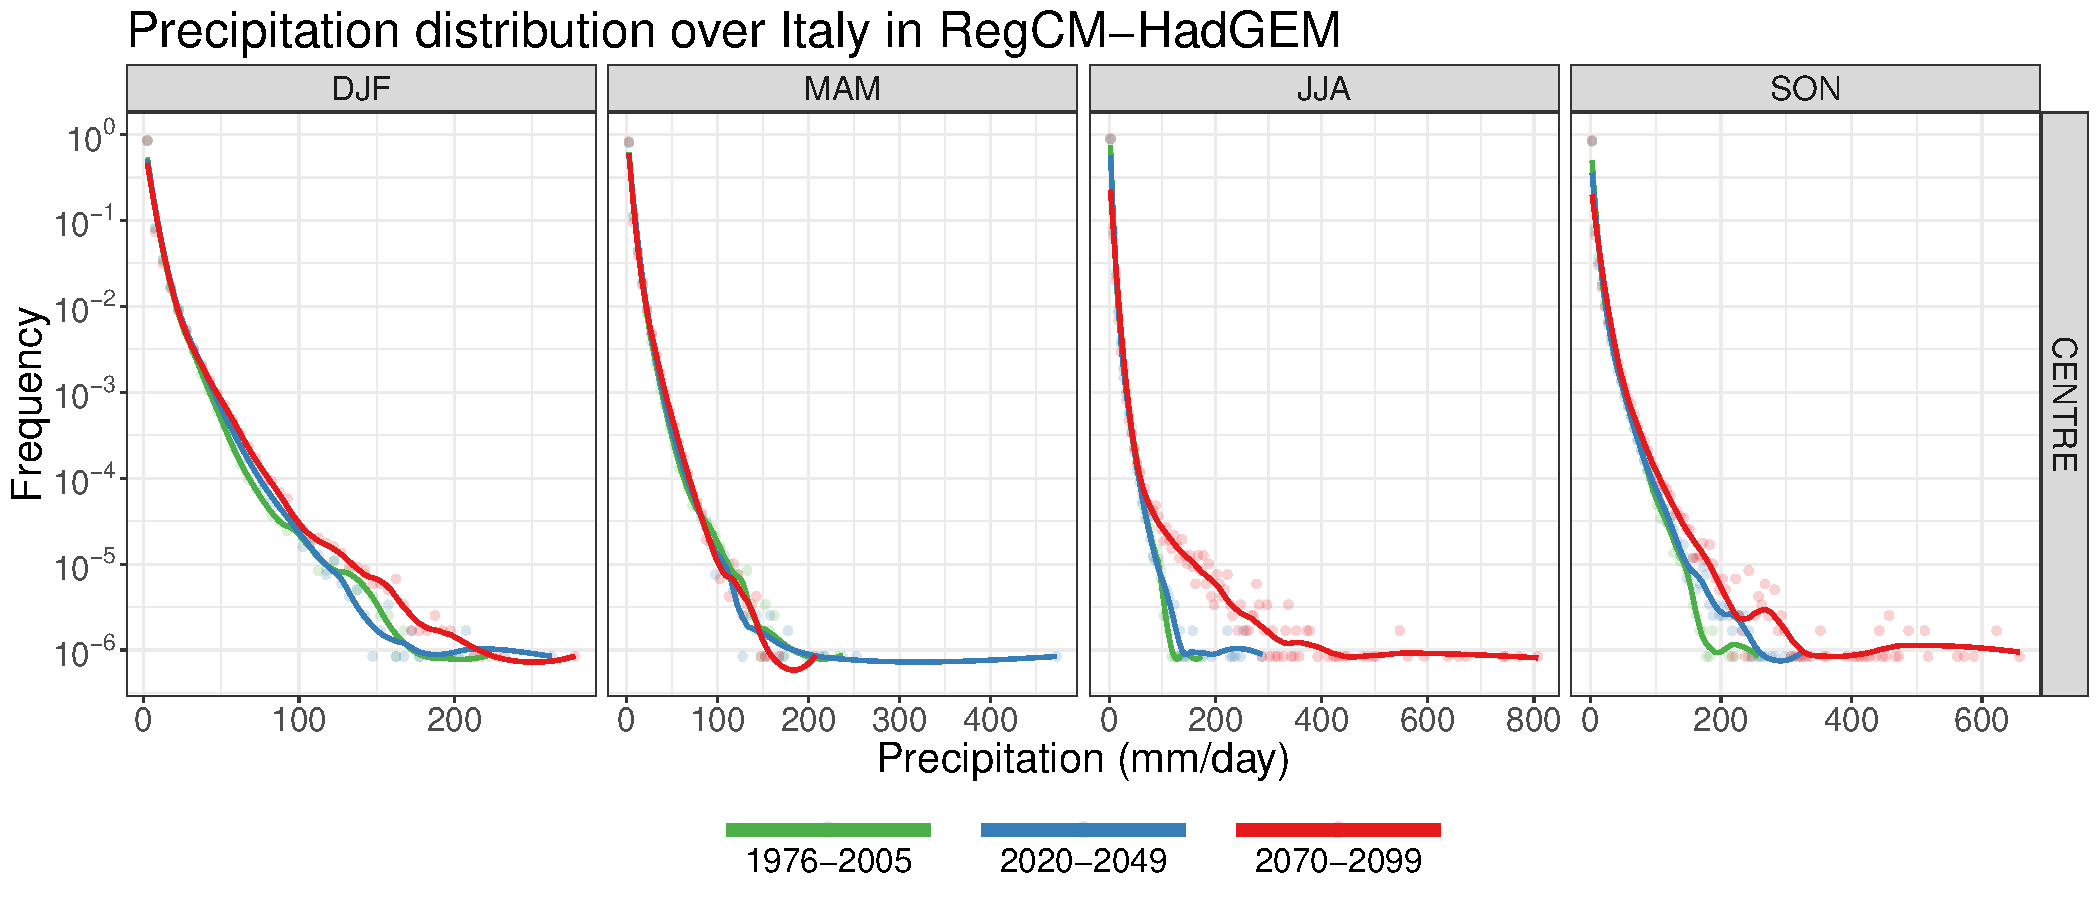
\includegraphics[width=0.8\textheight]{figures/change_rcm/pr/pdf_CENTRE_lines}
    \caption[Projected change of RegCM precipitation PDFs (1)]{
        Daily precipitation Probability Density Functions for the three timeslices of RegCM-HAD for the North and Centre regions. The solid lines are smoothed fits.
    }\label{fig:change_rcm_pr_pdf1}
\end{sidewaysfigure}
\afterpage{\clearpage}
\begin{sidewaysfigure}
    \centering
        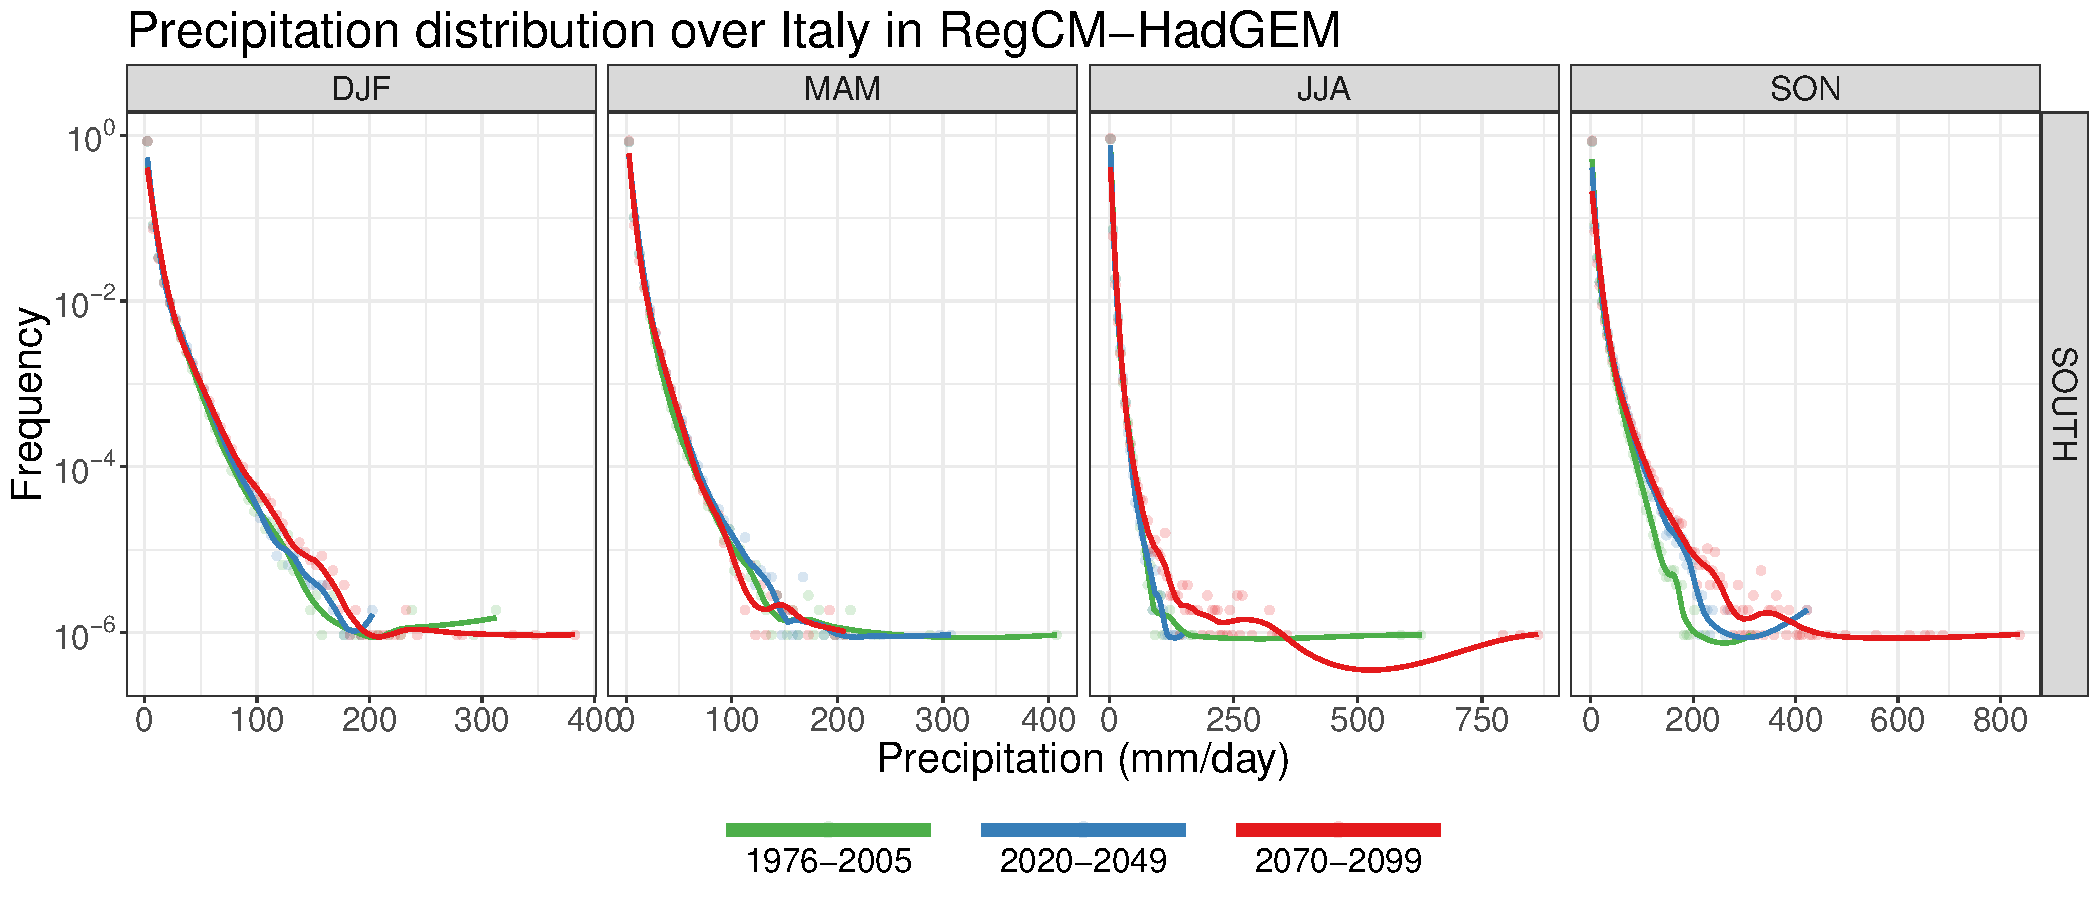
\includegraphics[width=0.8\textheight]{figures/change_rcm/pr/pdf_SOUTH_lines}
        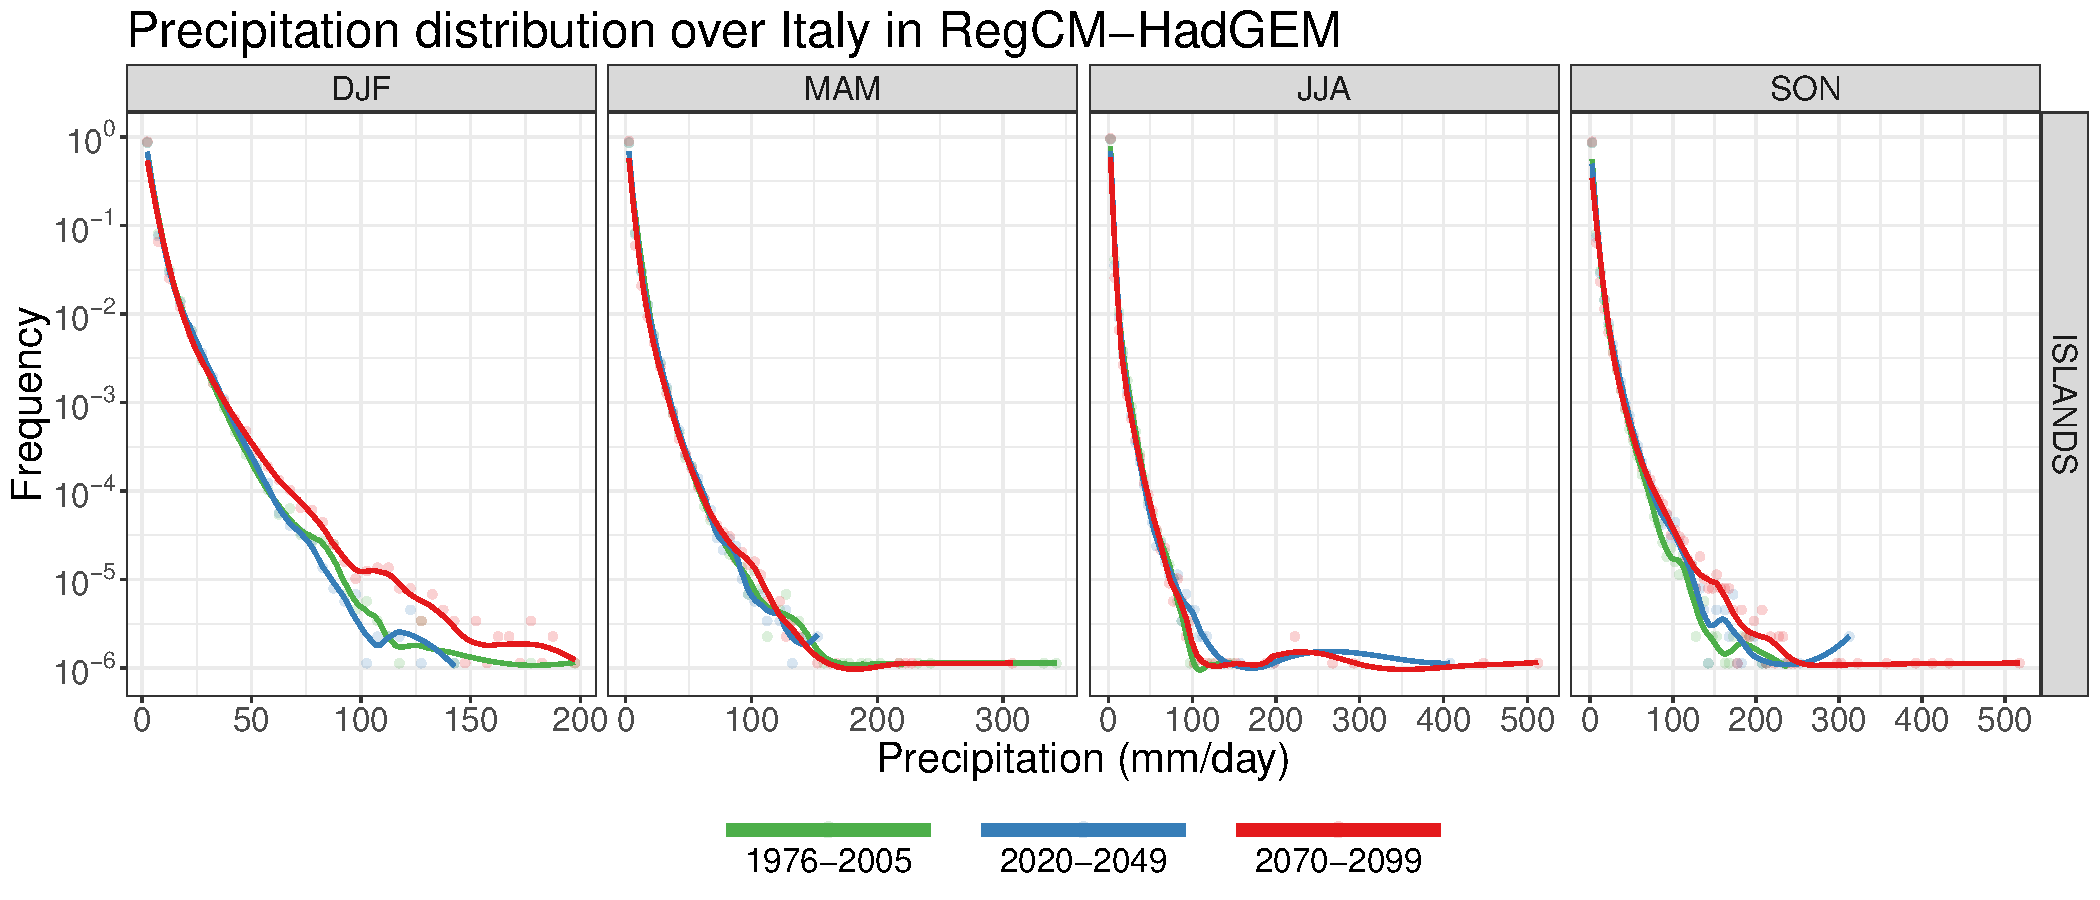
\includegraphics[width=0.8\textheight]{figures/change_rcm/pr/pdf_ISLANDS_lines}
    \decoRule
    \caption[Projected change  of RegCM precipitation PDFs (2)]{
        As \cref{fig:change_rcm_pr_pdf1}, but for the South and Islands regions.
    }\label{fig:change_rcm_pr_pdf2}
\end{sidewaysfigure}

Results on extreme temperature are deferred to \cref{appendix_tas}. The changes are mainly limited to an overall, spatially uniform increase in temperature of about 4 and \SI{6}{\celsius} in winter and summer respectively.


\section{The Italian hydrology in the three CHyM simulations} \label{sec:results_chym}
The findings of \cref{sec:change_rcm}, which indicate a general increase in extreme precipitation over Italy by the end of the century, can be linked to a change in flood hazard over all domains.
In the upcoming sections, we'll look at the performance of the CHyM model and discuss how the the projected changes in discharge extremes can be linked to the changes in precipitation. Following the literature \citep[e.g.][]{Alfieri2015a}, this is accomplished through several metrics.
For the comparison of CHyM simulation with station data, we used the following metrics:
\begin{description}[labelwidth=0pt, leftmargin=!, align=right]
    \item[SDH] Synthetic Design Hydrographs, derived from models and observations via the statistical procedure described in \cref{sec:3_mod_apprach}.
    \item[KGE] Kling-Gupta efficiency, a metric for analysing model efficiency similar to the Nash-Sutcliffe coefficient, devised by \citet{Gupta2009} and \citet{Kling2012}. Varies between $-\inf$ and $1$, with values closer to $1$ meaning better performance.
    \item[d] Index of agreement, a standard metric for assessing model performance by \citet{Willmott1984}. Varies between $0$ and $1$, with $0$ meaning no agreement and $1$ perfect match.
    \item[r] Pearson correlation coefficient; varies between $-1$ and $1$.
\end{description}
For evaluation of future change in average and extreme discharges, the following four metrics will be used:
\begin{description}[labelwidth=0pt, leftmargin=!, align=right]
    \item[$\boldsymbol{\overline{Q}}$] Average discharge.
    \item[$\boldsymbol{Q_{ymax}}$] Average maximum discharge calculated over each year in the given record.
    \item[$\boldsymbol{Q_{RP}}$] Projected peak discharge for the given Return Period $RP$, obtained by fitting a Gumbel distribution to the discharge data (see \cref{sec:3_mod_apprach}).
    \item[POT] Peak Over Threshold, the number of times (or fraction of timesteps) a discharge climatology surpasses a given threshold, usually given by the $Q_{RP}$ for a given Return Period.
\end{description}
The last three metrics, which represent extreme discharges, are chosen in order to act as proxies for flood events.

%------------------------------------
%	CHYM VALID
%------------------------------------
\subsection{Validation of the CHyM simulations}
The three CHyM simulations are here validated.
The two simulations CHyM-OBS and CHyM-ERA, driven by GRIPHO and RegCM-ERA, can be compared directly to the available discharge data (\cref{sec:disch_obs}) with standard metrics mentioned in the the beginning of this chapter.
Unfortunately, due to the low station availability (both in number of stations and length of the timeseries), most domains contain few or no discharge stations sharing a long enough period with the CHyM simulations.
The validation is thus carried out only for the two domains where station availability is more complete (the Po basin and Central Italy).
The results are, however, affected by the low quality of the provided observed discharge data, which present several irregularities, inhomogeneities and suspicious values.

For brevity, only a few of the maps are shown here. %TODO add stuff in appendix
\Cref{fig:valid_q_gripho_reg1} shows the index of agreement and Kling-Gupta efficiency for the GRIPHO-driven simulation over the Po basin, which is the largest basin in Italy.
Both metrics show good agreement with observations in most of the domain except the northernmost stations, located in Switzerland. This is also confirmed by the correlation (not shown), which is higher than 0.6 for most stations.
Larger basin tend to perform better better in these metrics.\\
Results in Central Italy (see \cref{fig:valid_q_gripho_reg3} for the index of agreement and the correlation) show generally acceptable performance for the GRIPHO-driven simulation.
Nevertheless, several stations in the eastern part of the domain indicate correlation values smaller than 0.5, suggesting that the model is not performing as good as before in this part of the domain.
This is also confirmed by the other metrics.
However, the Tevere river basin, which is the main catchment of the region, is showing good results in all metrics.
\begin{figure}
    \centering
    \begin{subfigure}{0.8\textwidth}
        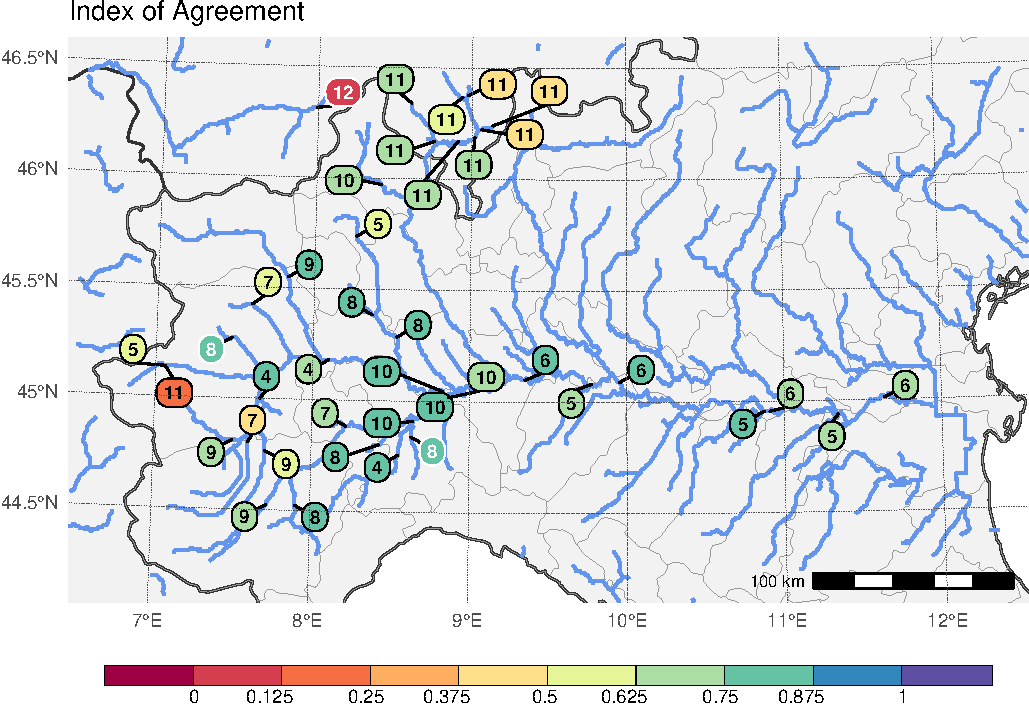
\includegraphics[width=\textwidth]{figures/valid_Q/metrics/intdb-fil-nc_reg1_22_d}
    \end{subfigure}\\
    \begin{subfigure}{0.8\textwidth}
        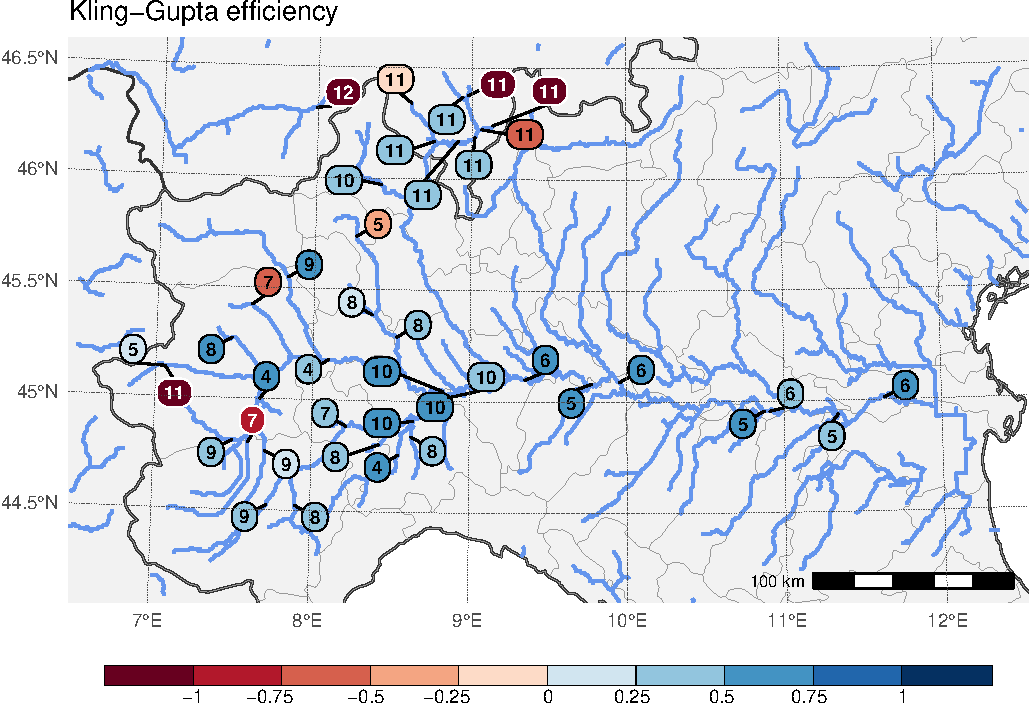
\includegraphics[width=\textwidth]{figures/valid_Q/metrics/intdb-fil-nc_reg1_22_KGE}
    \end{subfigure}
    \decoRule
    \caption[CHyM (GRIPHO) performance metrics for the Po basin]{
        Index of agreement (top) and Kling-Gupta Efficiency (bottom) for the CHyM simulation driven by GRIPHO over the Po basin, compared with observations. Colours indicate the value of the metric, numbers the total length of the time period in common with observations (in years).
    }\label{fig:valid_q_gripho_reg1}
\end{figure}
\begin{figure}
    \centering
    \begin{subfigure}{0.7\textwidth}
        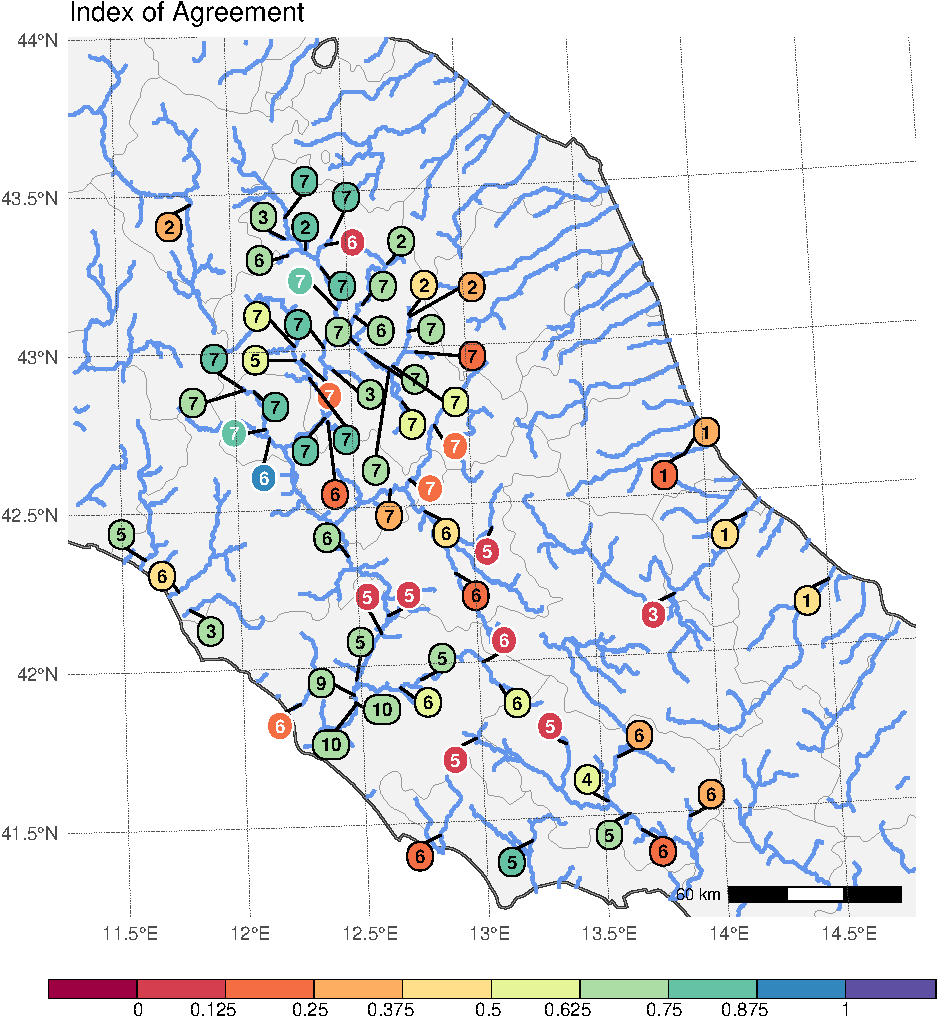
\includegraphics[width=\textwidth]{figures/valid_Q/metrics/intdb-fil-nc_reg3_22_d}
    \end{subfigure}\\
    \begin{subfigure}{0.7\textwidth}
        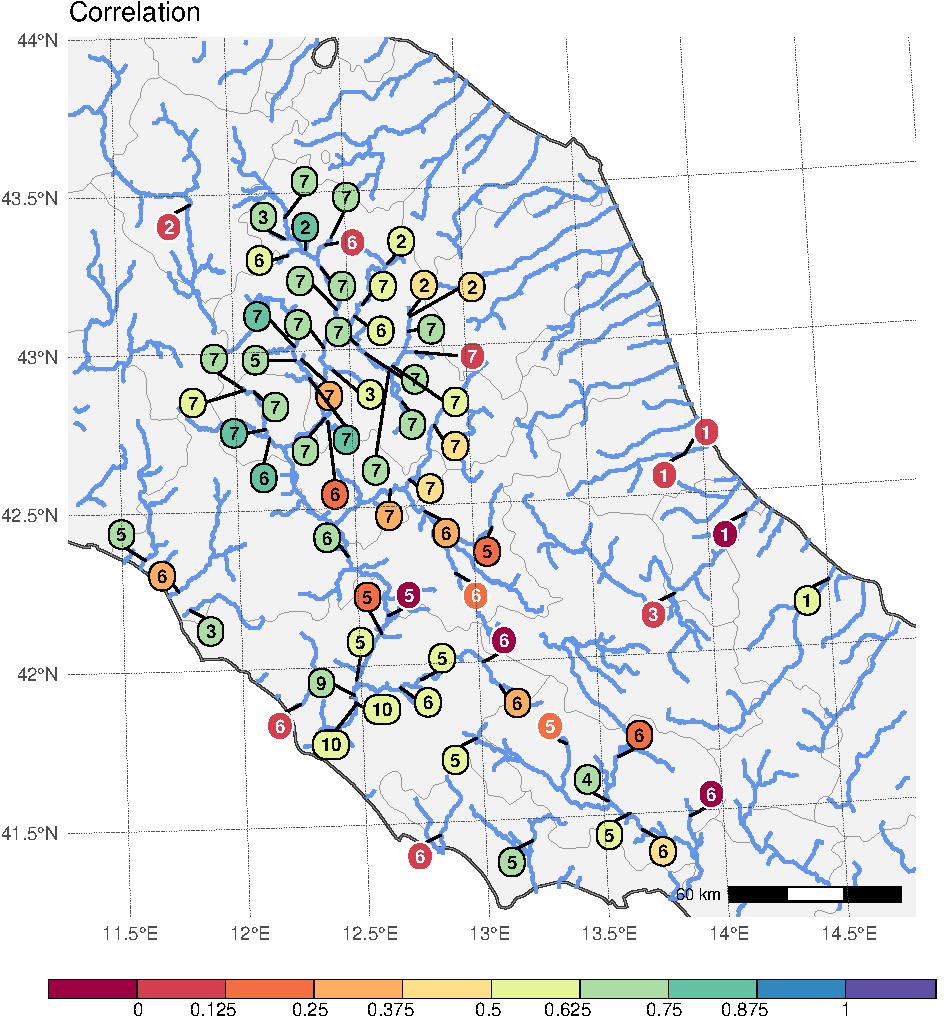
\includegraphics[width=\textwidth]{figures/valid_Q/metrics/intdb-fil-nc_reg3_22_r}
    \end{subfigure}
    \decoRule
    \caption[CHyM (GRIPHO) performance metrics for Central Italy]{
        Index of agreement (top) and correlation (bottom) for the CHyM simulation driven by GRIPHO over Central Italy, compared with observations. Colours indicate the value of the metric, numbers the total length of the time period in common with observations (in years).
    }\label{fig:valid_q_gripho_reg3}
\end{figure}

In regional climate simulations, even if laterally driven by reanalysis, the timing and intensity of heavy precipitation events, which is crucial for a proper representation of discharge, can be quite different from reality.
This is reflected by the worsening of 
% For this reason, in the CHyM simulation driven by RegCM-ERA the discharge over the two domains is not as well reproduced:
correlation and KGE values in RegCM-ERA (\cref{fig:valid_q_regcm}) are still mostly positive, but generally low.
The Po river basin, which, due to its large size, is less sensitive to precipitation timing, is the one which is better reproduced.
\begin{figure}
    \centering
    \begin{subfigure}{0.7\textwidth}
        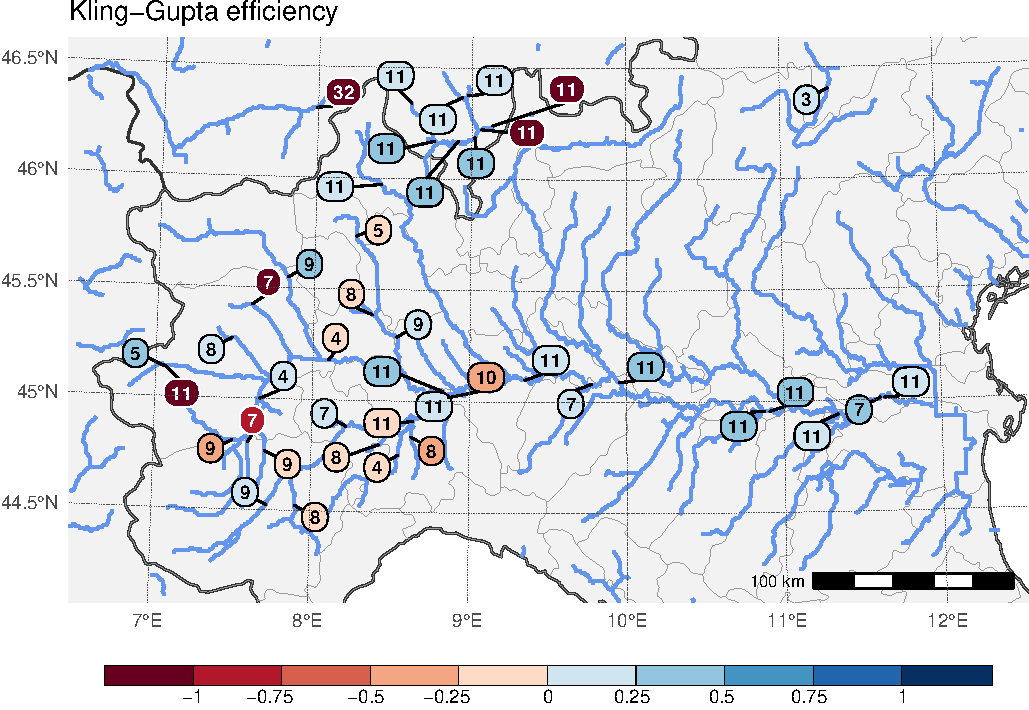
\includegraphics[width=\textwidth]{figures/valid_Q/metrics/regcm-nn_reg1_22_KGE}
    \end{subfigure}\\
    \begin{subfigure}{0.7\textwidth}
        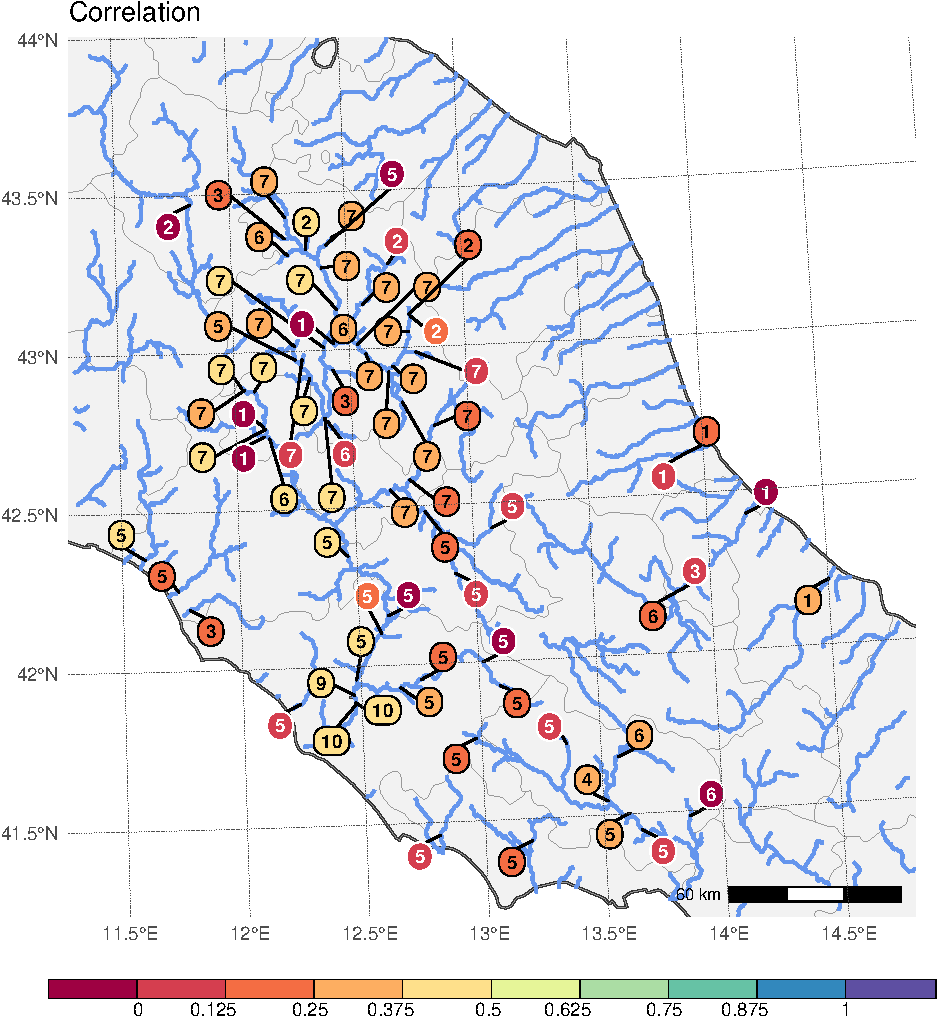
\includegraphics[width=\textwidth]{figures/valid_Q/metrics/regcm-nn_reg3_22_r}
    \end{subfigure}
    \decoRule
    \caption[CHyM (RegCM-HadGEM) performance metrics]{
        Kling-Gupta Efficiency (top, over the Po basin) and index of agreement (bottom, over Central Italy) for CHyM-HAD, compared with observations. Colours indicate the value of the metric, numbers the total length of the time period in common with observations (in years).
    }\label{fig:valid_q_regcm}
\end{figure}

Validating the performance of CHyM-HAD, the CHyM simulation driven by RegCM-HAD, is more difficult.
In this case, since climate simulations do not represent real timing of the events, but rather only a statistical representation of it, no direct comparison with observations can be made.
One way to validate the simulations is to use the Synthetic Design Hydrographs that are computed by fitting yearly maxima to an extreme value distribution (see \cref{sec:3_mod_apprach} for details).
These Hydrographs, which represent the typical discharge timeseries of an extreme event, can be calculated for any river point and can be compared between two points with different time coverage, being them only a statistical representation of the discharge of a given river segment.
% This has the useful effect of increasing the number of available stations for the validation.
% even if the time periods available do not coincide with model runs, under the assumption that hydrology is stable and extreme value discrepancies between model and observations are only due to the model's performance.
This approach works best if a long timeseries of discharge data is available.
For CHyM model runs driven by RegCM at least 30 years are considered, while the simulation driven by GRIPHO has only 16 years of data.
The length of the time period for discharge observations from station data varies by station; only stations with more than 10 years of data are considered here.\\
\Cref{fig:example_sdhs_1,fig:example_sdhs_2} show Synthetic Design Hydrographs for selected stations, compared with CHyM-OBS, CHyM-ERA and CHyM-HAD.
The latter is shown across the three selected timeslices and is generally found to increase discharge by the end of the century; this topic will be more widely discussed in the next section.
In particular, \cref{fig:example_sdhs_1} shows SDHs for two selected stations in the Po river basin, which were initially used for testing the methodology. These stations are known to be reliable and relatively unaffected by upstream water management.
The three CHyM-OBS, CHyM-ERA and CHyM-HAD simulations show here similar results to the observations for the present day, but an overestimation in the peak discharge at the Isola Sant'Antonio Po station can be found in the CHyM-OBS and CHyM-ERA simulations.
\Cref{fig:example_sdhs_2} shows instead example SDHs for two stations in Central Italy, characterised by widely different drained areas (16361 and \SI{53}{\kilo\meter\squared}).
In both cases, peak discharges are close to those obtained from observations.\\
Model performance across different basin sizes is good, albeit, on average across all stations, an overestimation of peak discharges if generally found to be present in all simulations.
% It is impossible here to show the hydrographs for all domains for all stations: \cref{fig:QRP_bias} represents the median of the percentage bias between the peak 100-year discharge ($Q_{100}$, which is the maximum peak of the SDH for the 100-year Return Period) as obtained from stations and from model simulations.
% All three historical simulations tend to overestimate the value of the peak discharge; this overestimation is larger in CHyM-OBS, and smaller in CHyM-HAD.
% Of the nine regions, peak discharges in North-Eastern Italy are the most overestimated (up to $+600\%$), while Central-Northern Italy is even slightly underestimated in the HadGEM simulation ($-7\%$).
% Due to the statistical nature of the $Q_{RP}$ metric, the results for other Return Periods do not differ from those of $Q_{100}$.
This might partially be due to the fact that discharge rating curves generally tend to underestimate extreme flows \citep{DiBaldassarre2009}.
\afterpage{\clearpage}
\begin{sidewaysfigure}
    \centering
        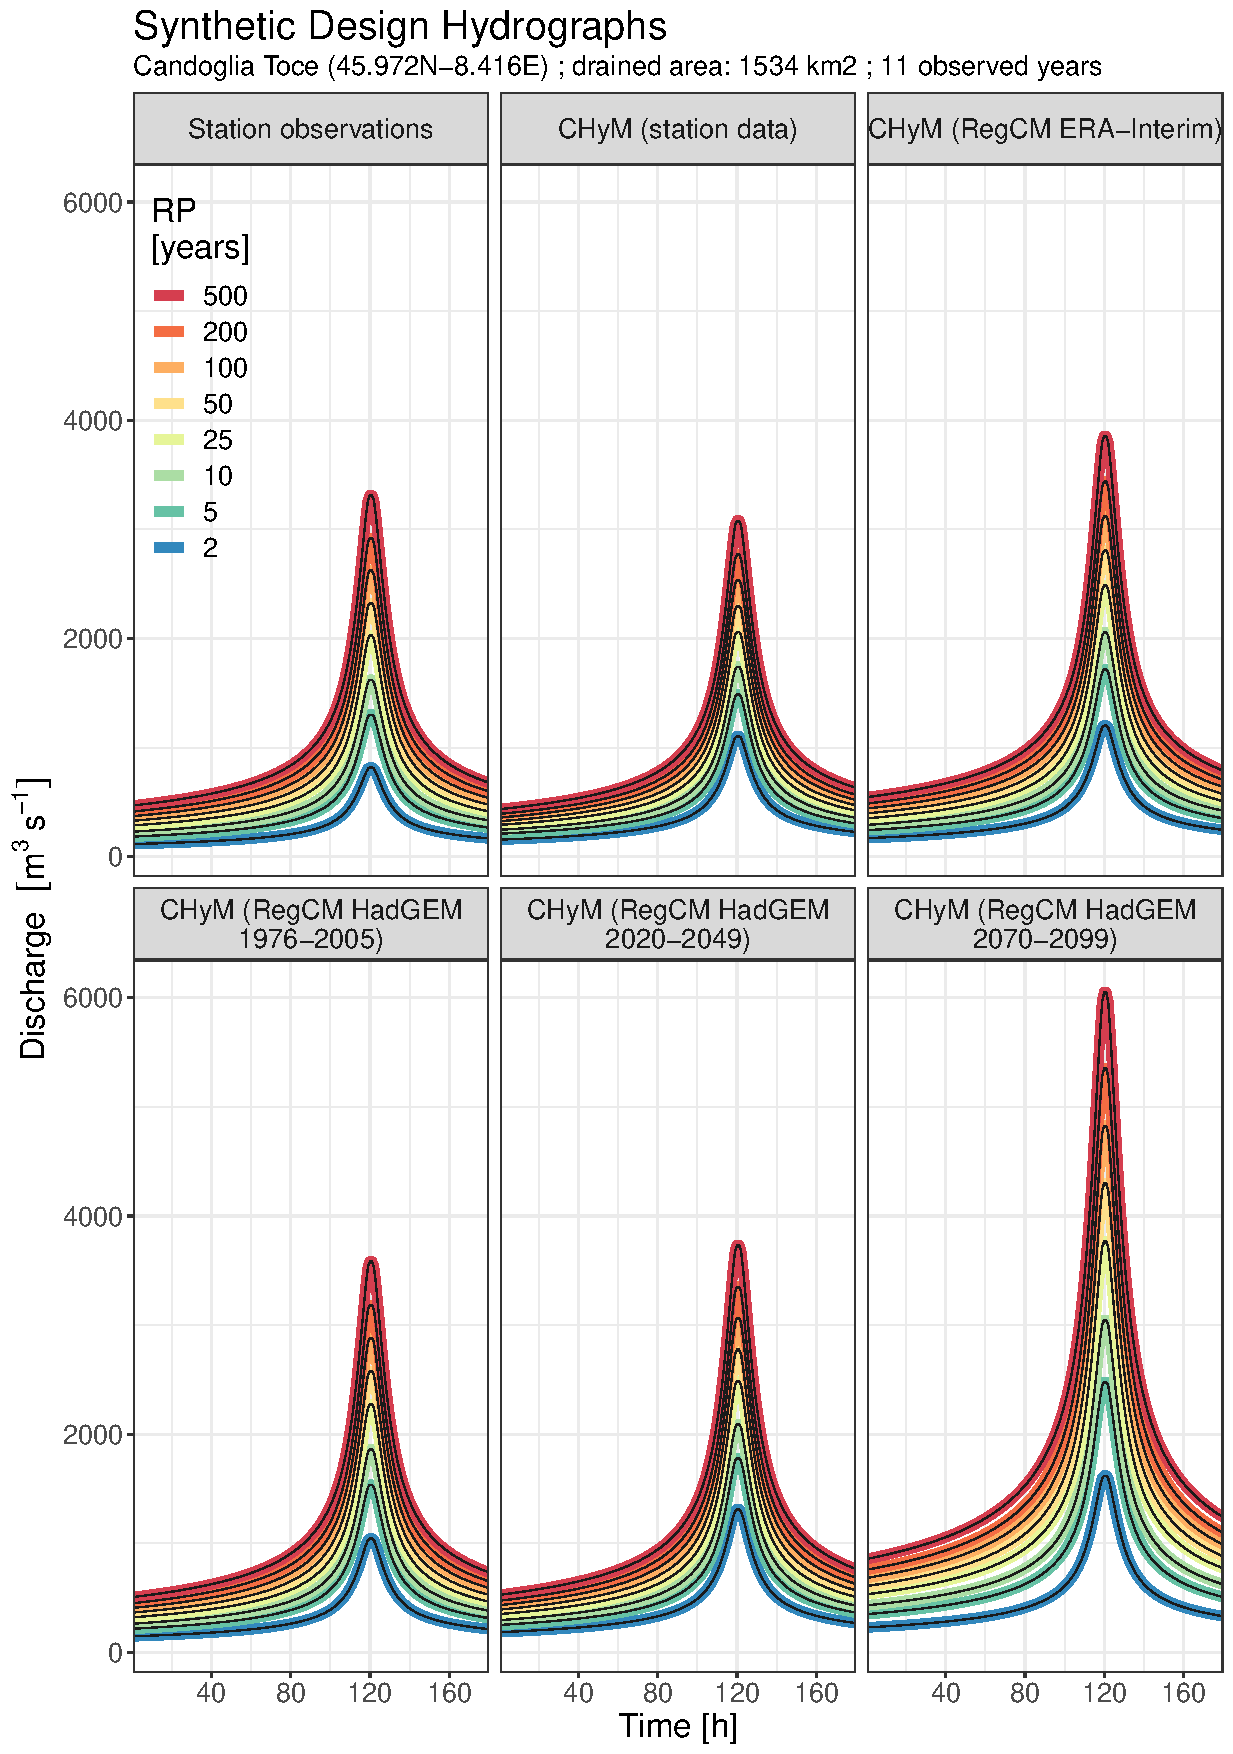
\includegraphics[width=0.45\textheight]{figures/valid_Q/SDH/id4_SDH_reg1_22}
        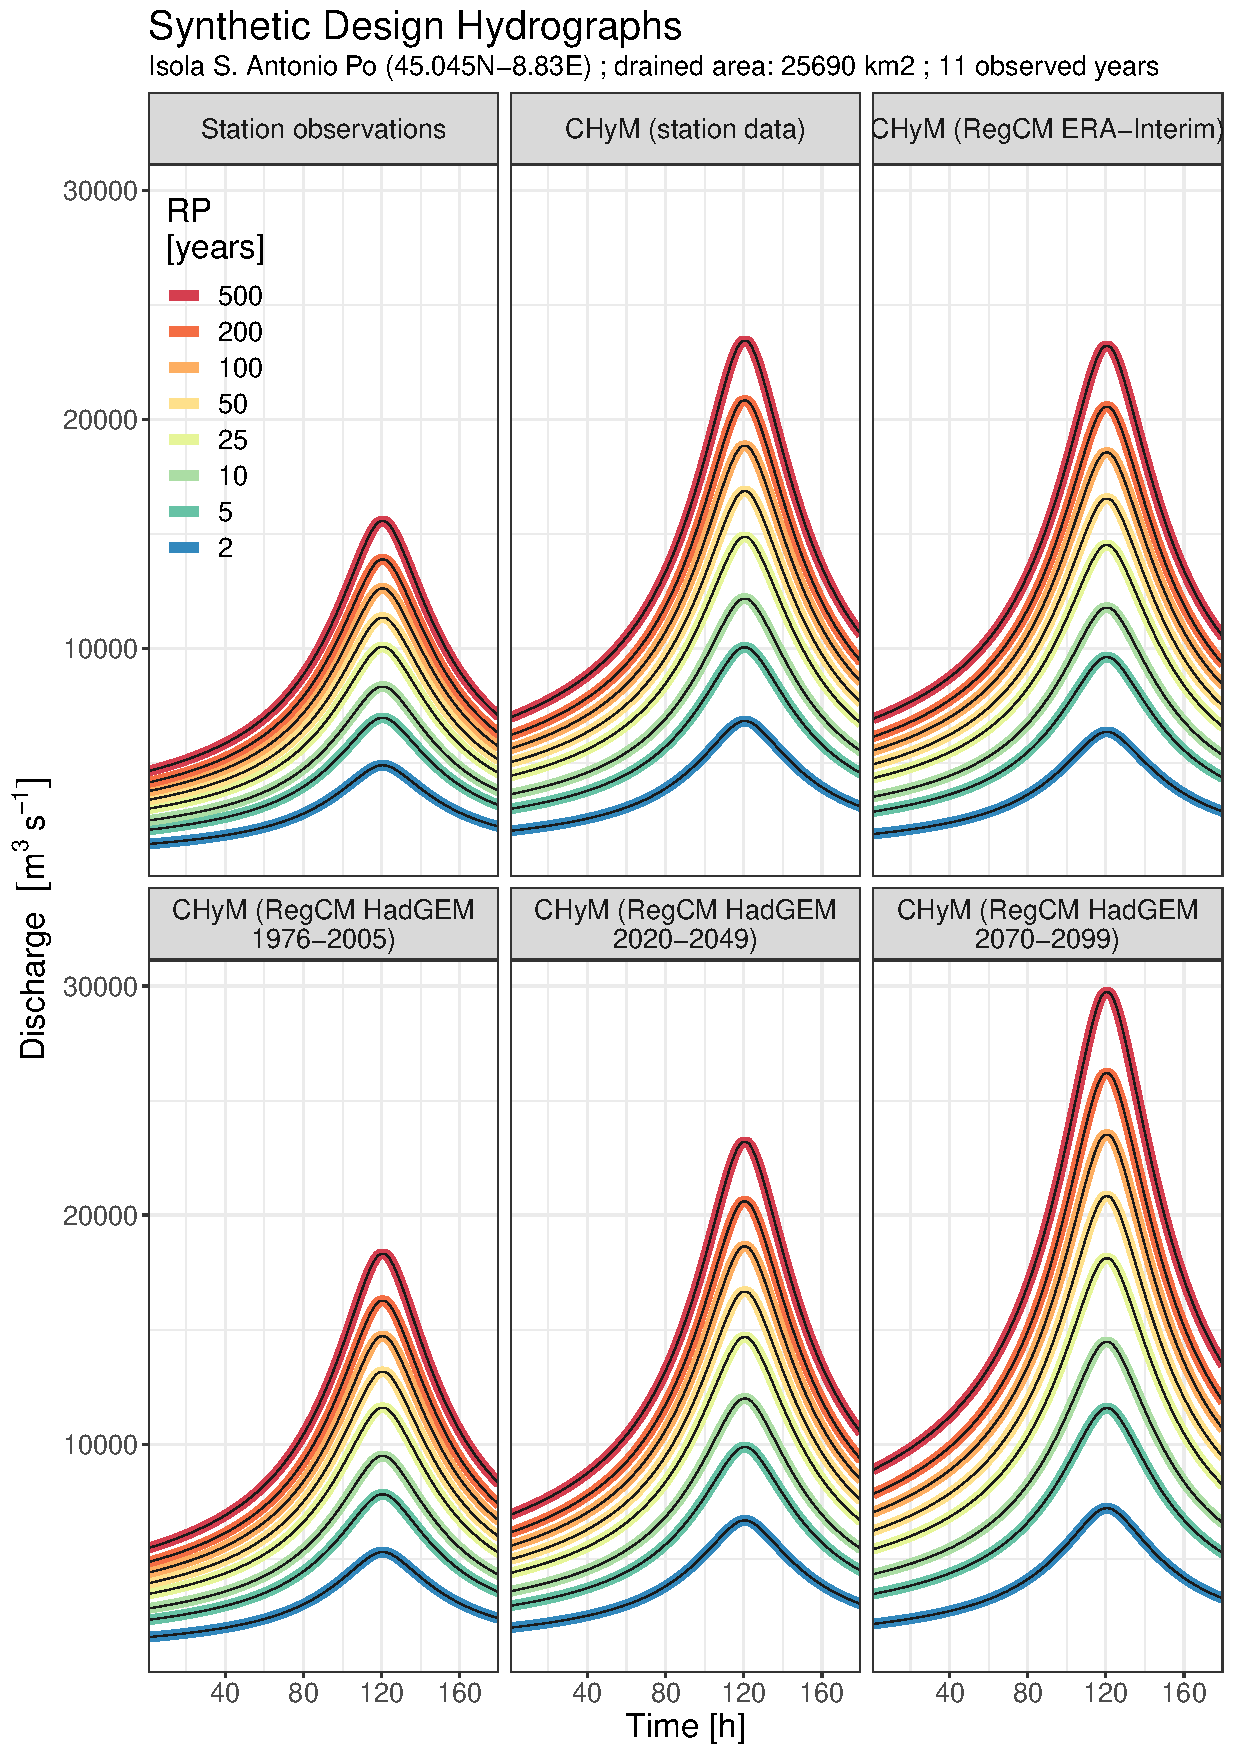
\includegraphics[width=0.45\textheight]{figures/valid_Q/SDH/id12_SDH_reg1_22}
    \decoRule
    \caption[Example SDHs (1)]{
        Example SDHs for two station locations in the Po basin. These stations were among the ones used for the initial definition of the methodology.
    }\label{fig:example_sdhs_1}
\end{sidewaysfigure}
\afterpage{\clearpage}
\begin{sidewaysfigure}
    \centering
        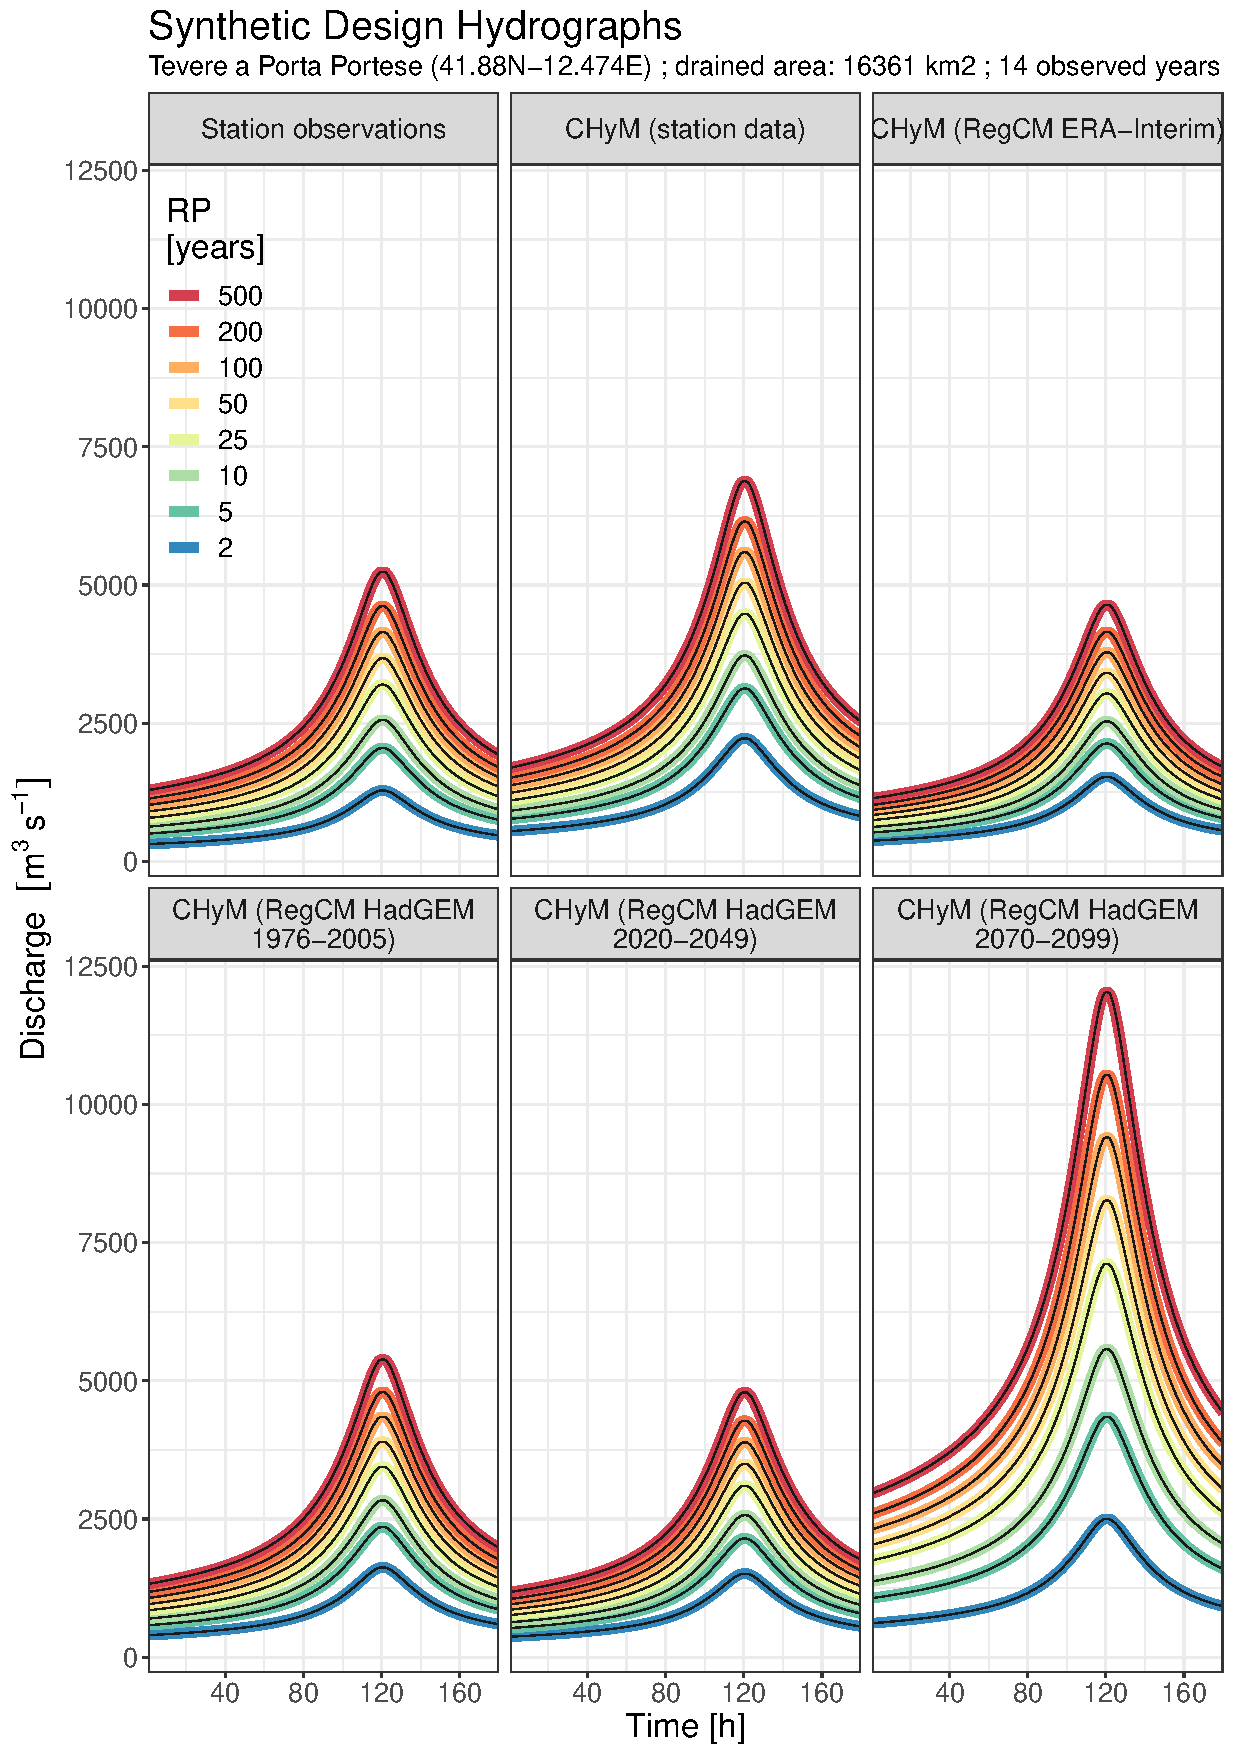
\includegraphics[width=0.45\textheight]{figures/valid_Q/SDH/id57_SDH_reg3_22}
        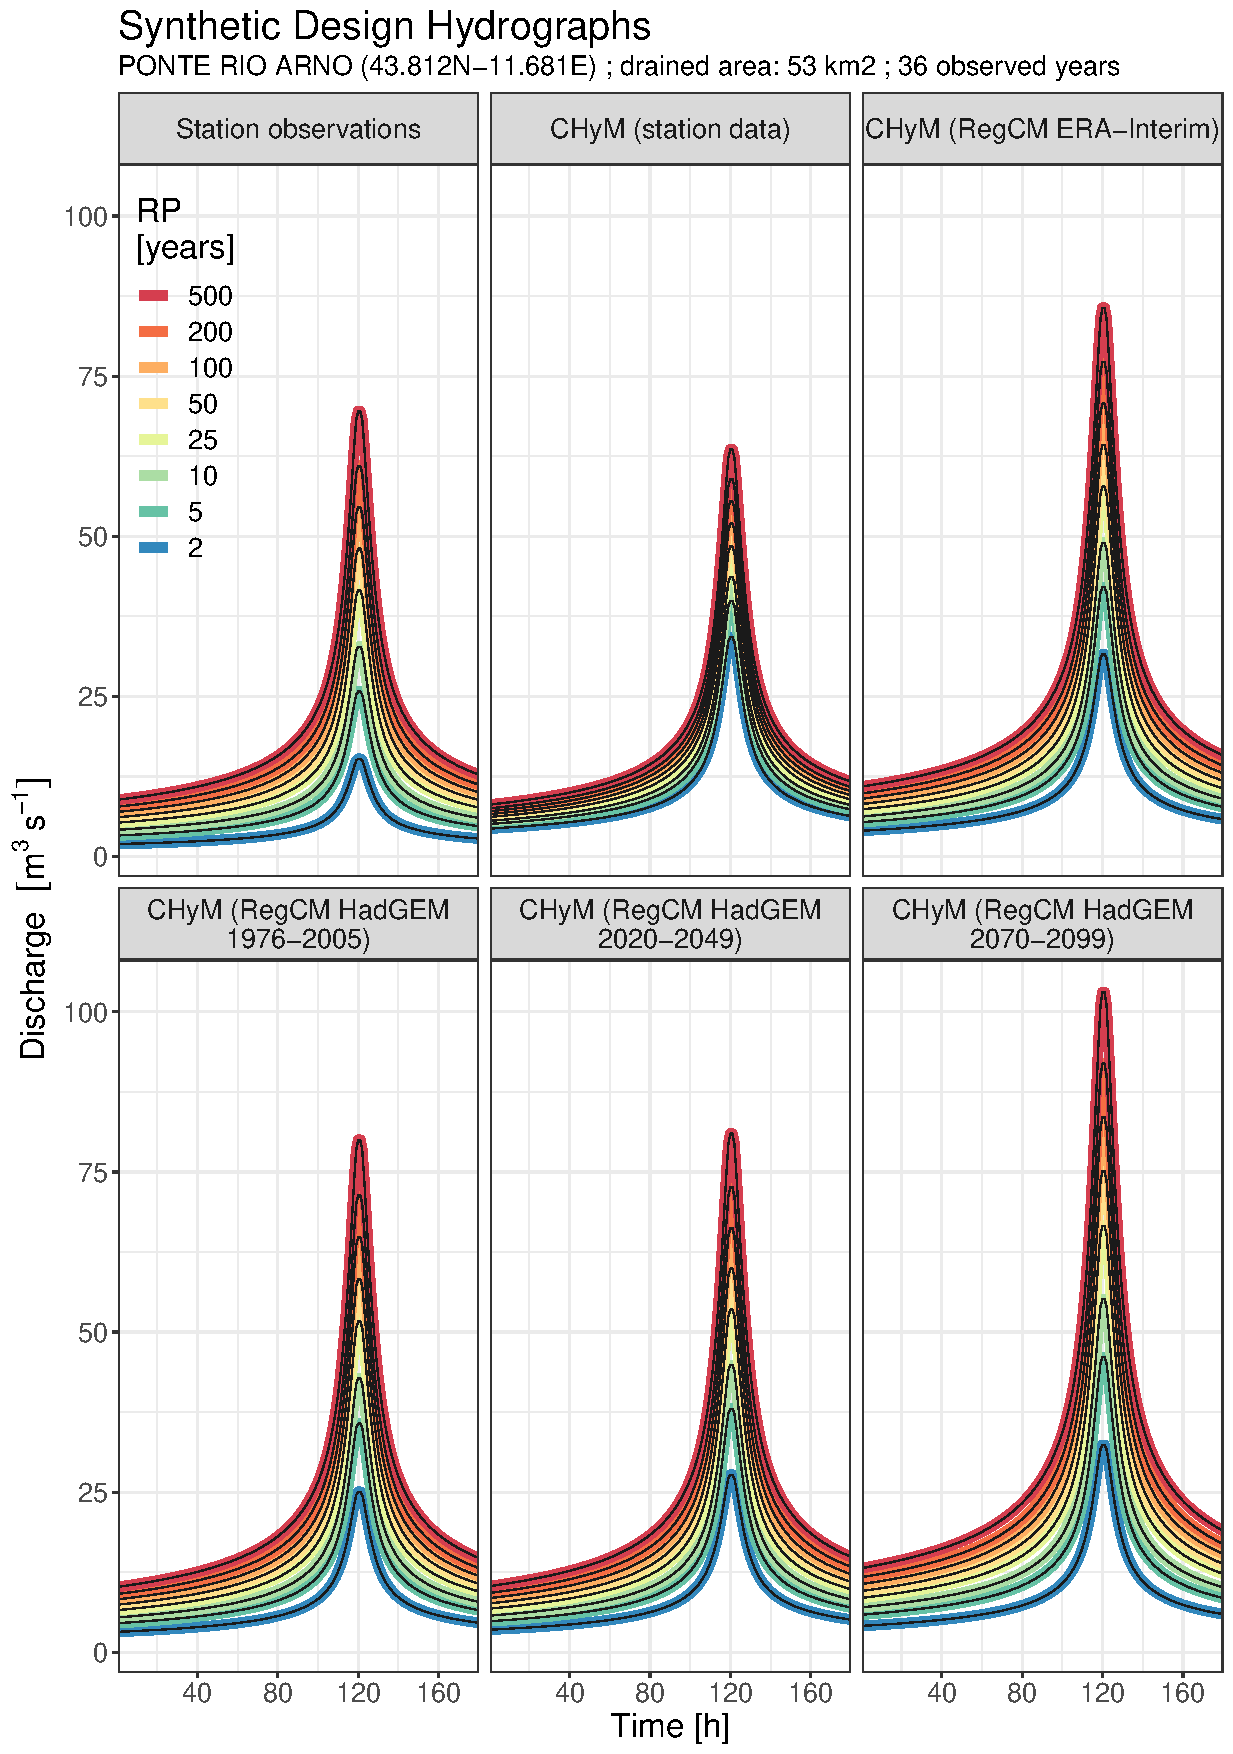
\includegraphics[width=0.45\textheight]{figures/valid_Q/SDH/id81_SDH_reg9_22}
    \decoRule
    \caption[Example SDHs (2)]{
        Example SDHs for two station locations in Central Italy with drastically different basin sizes.
    }\label{fig:example_sdhs_2}
\end{sidewaysfigure}

% \begin{figure}
%     \centering
%     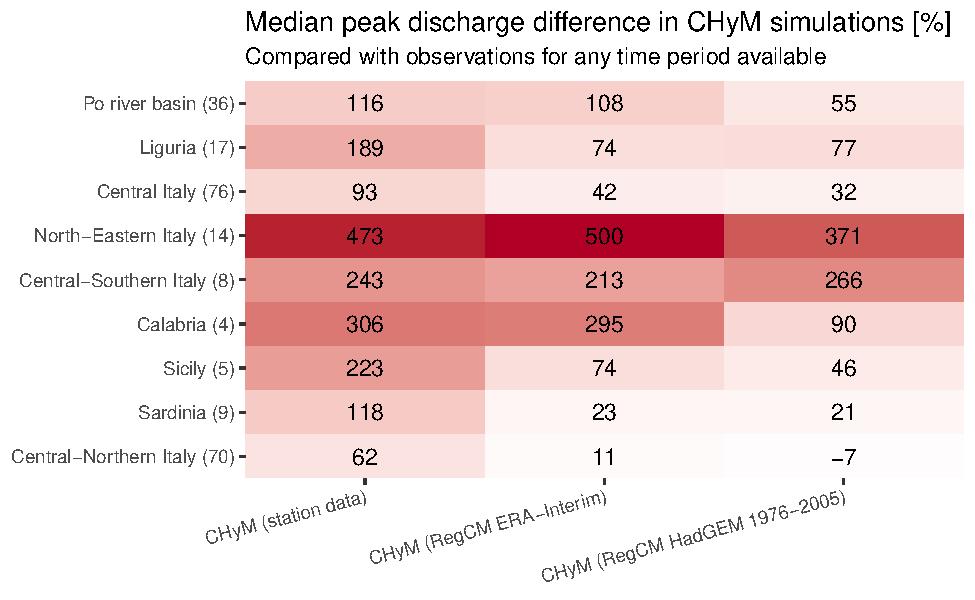
\includegraphics[width=0.7\textwidth]{figures/valid_Q/peakQ_bias_change}
%     \decoRule
%     \caption[$Q_{100}$ bias with observations in the CHyM simulations]{
%         $Q_{100}$ bias with observations in the three CHyM simulations, for each domain. The number of stations considered for each domain is indicated in parenthesis next to the domain label, on the Y axis. Stations with less than 10 years of data were excluded.
%     } \label{fig:QRP_bias}
% \end{figure}

%------------------------------------
%	CHYM CHANGE
%------------------------------------
\subsection{Future changes in mean and extreme discharges over Italy}
The CHyM-HAD simulation, which covers the period 1975 to 2100, allows us to analyse the possible changes in discharge in a future climate scenario.
% perform change analysis of a possible future scenario.
% \Cref{fig:} shows changes in the annual cycle of TODO ... they are weird???
In \cref{fig:change_qmean_hadgem}, the change in average discharge between the two future timeslices and the reference period is shown for the nine domains used to cover the complete Italian territory.
Average discharges obtained from the CHyM-OBS, also plotted as a reference, show good agreement with CHyM-HAD, which covers a similar period of time.
Increases (decreases) in mean discharge are larger in the North in winter (summer), which can be directly linked to the changes in mean precipitation (\cref{fig:change_rcm_pr_mean}) and snow melt \citep{coppola2014ChahydconPobasundglowar}.
By the end of the century, Central Italy is the only region which shows increased discharges in summer, except for the Tevere river, the main of the region.
In autumn in the far future, discharges increase all over Italy, especially for smaller rivers.
An exception is the Tevere, the principal river of the second largest Italian basin, which shows a negative change of about $25\%$. 
Both increasing and decreasing signals are on average stronger in the far future compared to the near future.
The general trends between the two periods are not linear: Sardinia, for example, shows decreased average summer discharges in the near future, but slight increases by the end of the century (despite decreasing precipitation); in autumn, average discharges increase over most of the country, despite little to no change in average precipitation. 
% TODO how is this possible WTF?
\begin{figure}
    \centering
    \includegraphics[width=\textwidth]{figures/change_Q/Qmean_ITA_4col_pctl}
    \decoRule
    \caption[Average discharge change in CHyM (HadGEM)]{
        Average discharge for CHyM-OBS and CHyM-HAD (leftmost two columns) and percentage change for near and far future (leftmost two columns), over the four seasons. To avoid overlaps and overplotting, only the basins completely enclosed in each of the nine simulation domains are plotted and only the major rivers are shown for each basin.
    } \label{fig:change_qmean_hadgem}
\end{figure}

As a basic metric for high discharge, the mean annual maximum discharge ($Q_{ymax}$) over the three selected 30-year periods is displayed in \cref{fig:change_qymax_hadgem}.
Compared to CHyM-OBS, in agreement with the RegCM results, CHyM-HAD for the reference period shows generally good performance, despite a slight underestimation for winter in the Po plain.
By the end of the century, maximum yearly discharges increase in winter and autumn across most of Italy, with changes often above $+50\%$.
In summer and spring, results are more mixed and depend on the region: central Italy shows an increase in summer (including the Tevere river basin, contrarily to mean discharge), while areas such as Sardinia and the Alps show a slight decrease in the same season.
Once again changes by the end of the century are higher than in the near future and, in some cases (e.g. Central Italy), of opposite sign.
These changes can in general be linked to extreme precipitation changes in the driving model (\cref{fig:change_rcm_pr_r95}), which show similar patterns across the domain; there are however some notable differences, such as the marked decrease in 2070-2099 summer $Q_{ymax}$ over Sardinia (not mirrored by $\textrm{R95}_{ptot}$).\\
\begin{figure}
    \centering
    \includegraphics[width=\textwidth]{figures/change_Q/Qymax_ITA_4col_pctl}
    \decoRule
    \caption[Mean annual maximum discharge change in CHyM (HadGEM)]{
        Like \cref{fig:change_qmean_hadgem}, but for $Q_{ymax}$, the mean annual maximum discharge.
    } \label{fig:change_qymax_hadgem}
\end{figure}
\Cref{fig:change_qrp_hadgem} shows $Q_{RP}$: it is the peak projected discharge for the 2, 10, 20, 50 and 100 year Return Periods, calculated using the methodology described in \cref{sec:3_mod_apprach}.
Compared to the mean annual maximum discharge, this metric is more representative of extreme events, but it can only be computed on a yearly basis.
These extreme discharges are in line with CHyM-OBS or even somewhat underestimated for some rivers.
As for projections, in the near future changes appear to be relatively small and mixed across the domain; for the end of the century, instead, this metric shows a consistent increase in extreme discharges over the whole Italian territory, with only some areas (mainly in the southern region of Calabria) showing a slight decrease.
Some large rivers, such as the Po and the Tevere, show more than doubled values of the peak 100-year discharge, compared to 1976--2005.
The change results for the five Return Periods are almost identical, which is to be expected given the fact that the discharges are calculated using the same constant parameters, only changing the RP.
\begin{figure}
    \centering
    \includegraphics[width=0.8\textwidth]{figures/change_Q/QRP_ITA_4col_pctl}
    \decoRule
    \caption[Mean annual maximum discharge change in CHyM (HadGEM)]{
        Like \cref{fig:change_qmean_hadgem}, but for $Q_{RP}$, the peak projected discharge, calculated for 5 Return Periods: 2, 10, 20, 50 and 100 years.
    } \label{fig:change_qrp_hadgem}
\end{figure}
Another standard metric for extreme discharge is the number of times the discharge is higher than a chosen threshold. This Peak Over Threshold (POT) metric is calculated using as reference the peak projected discharge for different Return Periods (the same as in $Q_{RP}$,  \cref{fig:change_qrp_hadgem}).
Contrarily to the previous extreme metrics, this metric shows an overestimation on the side of CHyM-HAD compared to CHyM-OBS (\cref{fig:change_pot_hadgem}), which prompts for caution with drawing conclusions from this data.
The maps of POT change clearly show a strong increase in the frequency of future events, for each return period.
In particular, for the end of the century, the less frequent the event (more severe floods, higher Return Period), the higher the frequency increase: the frequency of exceedance of 100-year thresholds increases more than $500\%$ and up to tenfold over most of the domain, while the POT of 2-year events increases, on average, by a factor 2 or 3.
\begin{figure}
    \centering
    \includegraphics[width=0.8\textwidth]{figures/change_Q/POT_ITA_4col_pctl}
    \decoRule
    \caption[Peak over threshold change in CHyM (HadGEM)]{
        Like \cref{fig:change_qmean_hadgem}, but for number (and \% change) of Peak Over Threshold events above the relative $Q_{RP}$ (see \cref{fig:change_qrp_hadgem}) for 5 Return Periods: 2, 10, 20, 50 and 100 years.
    } \label{fig:change_pot_hadgem}
\end{figure}

Since floods are closely linked with extreme discharges, $Q_{ymax}$, $Q_{RP}$ and POT can all be considered proxies for flood events.
This simulation then unambiguously shows a strong increase in flood hazard towards the end of the century, if the current business-as-usual policy towards climate change is not subject to intervention.

%------------------------------------
%	CA2D RESULTS
%------------------------------------
\section{Flood hazard maps for the Italian territory}\label{sec:results_flood}
The CA2D hydraulic model is able to reproduce flood extent and water depth for the complete Italian domain, as described in \cref{sec:ca2d}.
Due to the lack of observational data, validation of CA2D against real inundation events is challenging.
As an example of validation, a case study was analysed by Rita Nogherotto from the ICTP Earth System Physic group: in November 2016 heavy rainfall over the north-west of Italy, and in particular in the regions of Piemonte and Liguria, led to increase of hydrometric levels over the danger thresholds for several rivers in the Po basin, such as the Bormida and the Tanaro.
The event caused vast damages and one casualty\footnote{For additional information about the event, refer to \url{https://it.wikipedia.org/wiki/Alluvione_del_Piemonte_del_2016} (in Italian)}. 
When utilising discharge data from CHyM-OBS, CA2D is able to reproduce with remarkable similarity the flooded extent as reported by COSMO-SkyMed satellite images, in \cref{fig:valid_casestudy}.
The actual flooded extents (top panels) are within the boundaries of the 100- and 500-year Return Period extents as simulated with the model (bottom panels) in both the areas considered.
This validation, although only partial, suggests the methodology described so far is reasonable.
\begin{figure}
    \centering
    \begin{subfigure}{7.3cm}
        \includegraphics[width=\textwidth]{figures/valid_flood/casestudy/overlay_flood-T500-all-box_obs}
    \end{subfigure}
    \begin{subfigure}{6cm}
        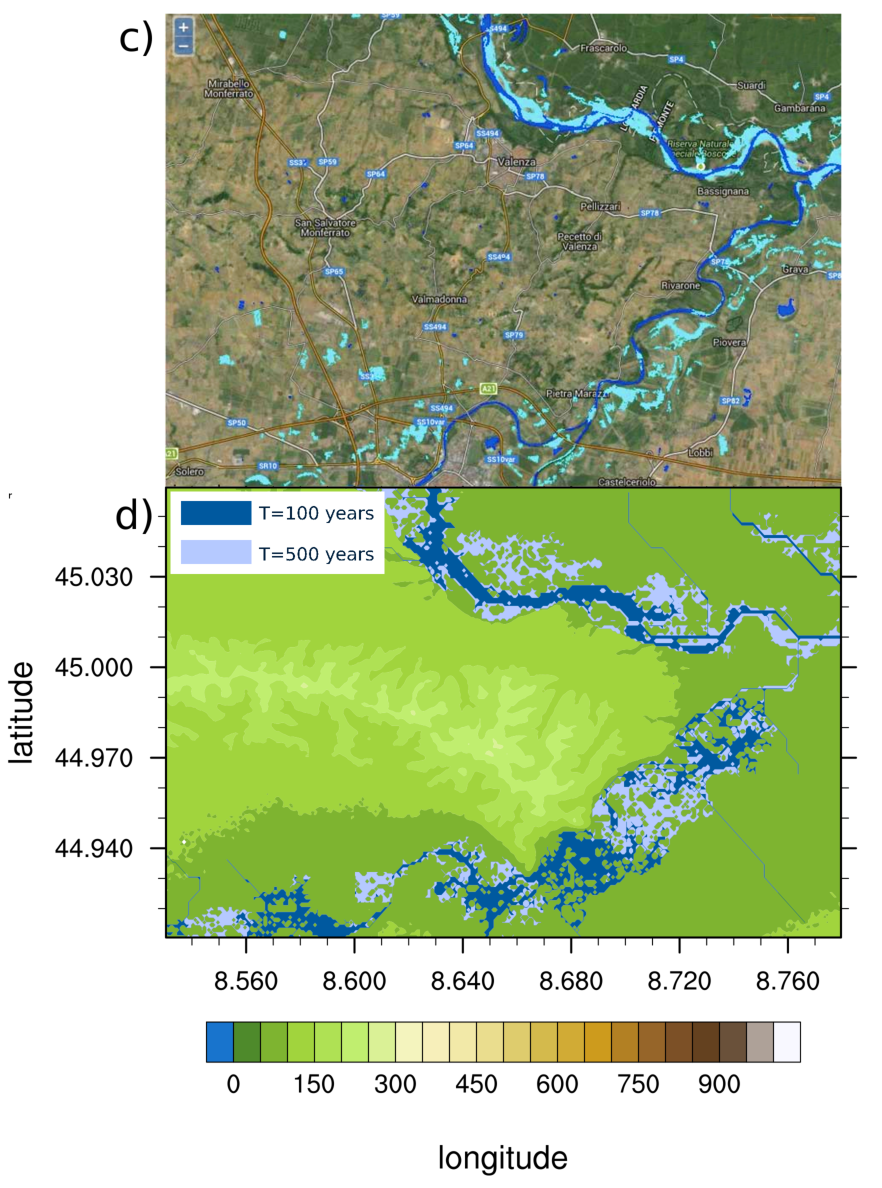
\includegraphics[width=\textwidth]{figures/valid_flood/casestudy/overlay_flood-T500-alessandria}
    \end{subfigure}
    \decoRule
    \caption[Case study: Piemonte 2016 flood]{
        Case study for the Piemonte 2016 flood, used for the validation of the methodology: left, an area south of Turin; right, close to Alessandria.
        The panels on top show the floods as acquired by the COSMO-SkyMed satellite constellation, while the lower panels show the flood as modelled by the integrated CHyM-CA2D method for Return Periods of 100 and 500 years. From \citet{nogherotto2019}, in preparation.
    }\label{fig:valid_casestudy}
\end{figure}

\Cref{fig:flooded_areas} shows preliminary results on flood hazard maps for the complete Italian territory and for four Peturn Periods (50, 100, 250 and 500 years), as reproduced by the CA2D model using discharge data from CHyM-OBS.
The results are similar to the official ISPRA flood maps (\cref{fig:ispra_ita_flood}), even though these maps tend to show a larger flooded extent compared to our product, in compatible Return Periods.
%TODO here I could plot both maps one on top of the other, or calculate the areas
However, the ISPRA maps are an ensemble of estimates obtained from the regional agencies, which might vary in quality and methodology.
The maps here produced are instead created via an approach based on a reproducible chain of high-resolution physical models.
These preliminary results are encouraging and lay the foundation for the future research avenues discussed in the next chapter.
\begin{figure}
    \centering
    % source of this data if you want to remake it:
    % /home/afantini/places/clima-archive4-b/ca2d_simulations/
    \begin{subfigure}{.49\textwidth}
        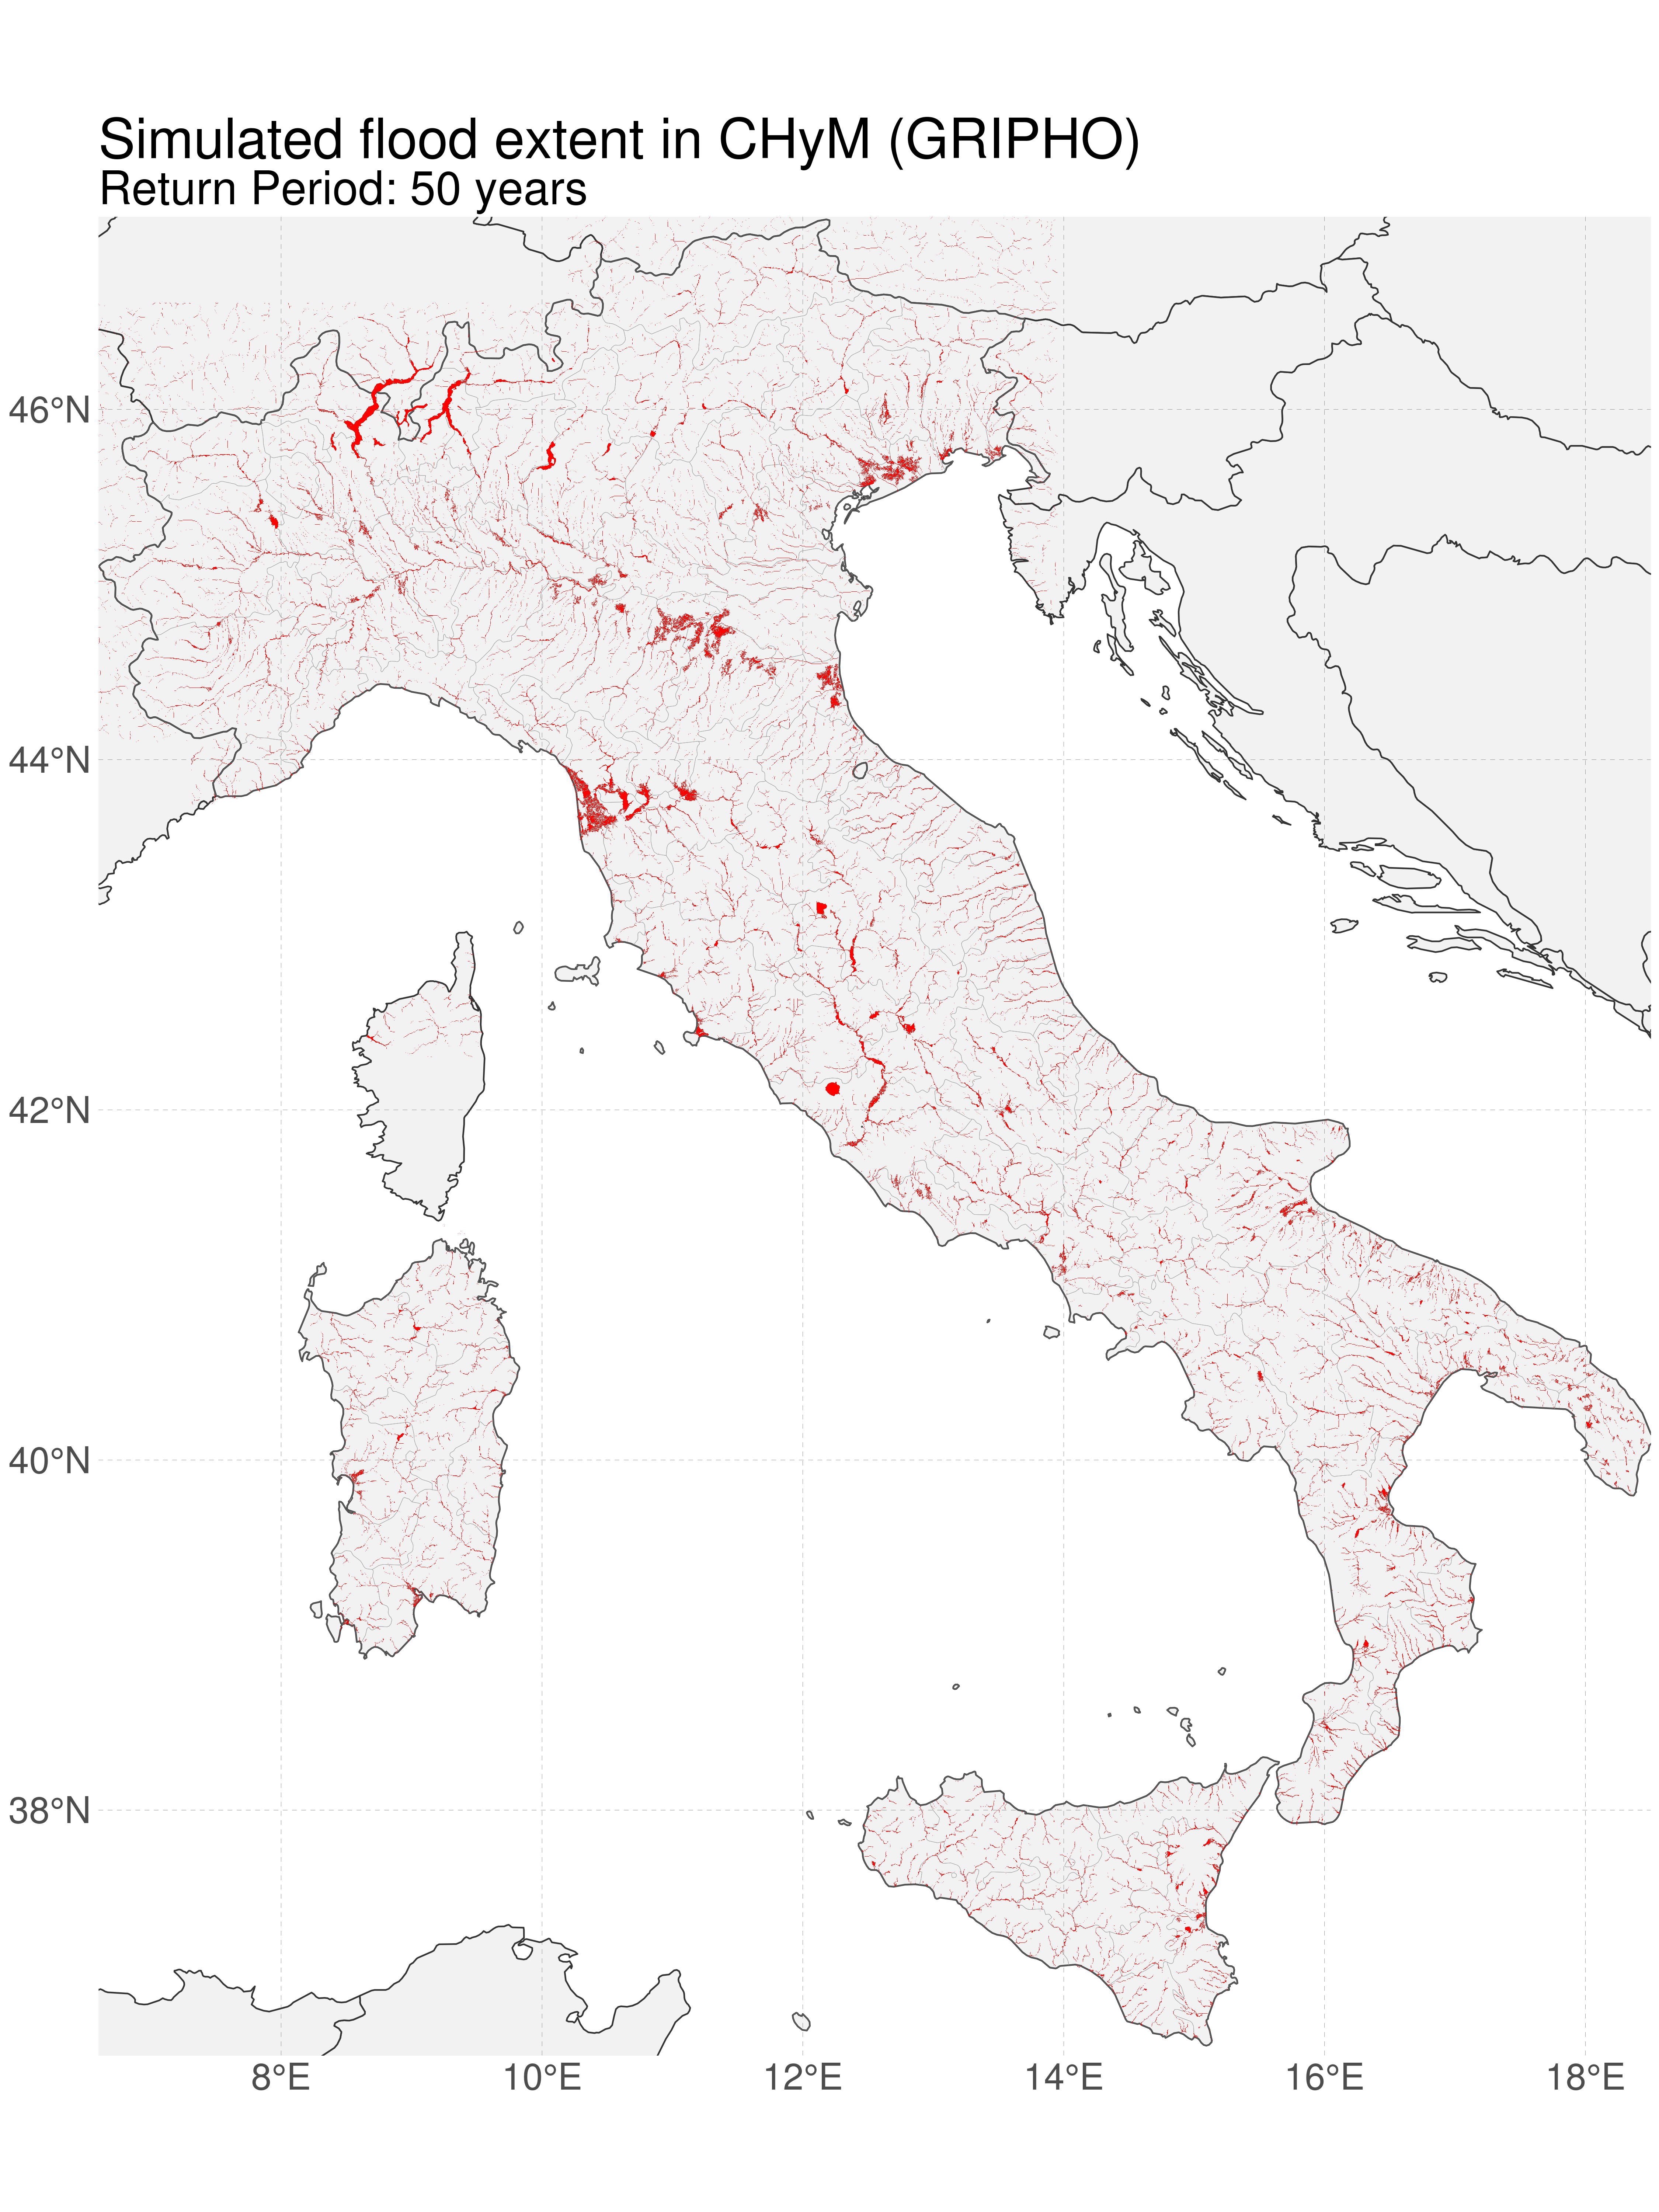
\includegraphics[width=\textwidth]{figures/valid_flood/flooded_areas/T50}
    \end{subfigure}
    \begin{subfigure}{.49\textwidth}
        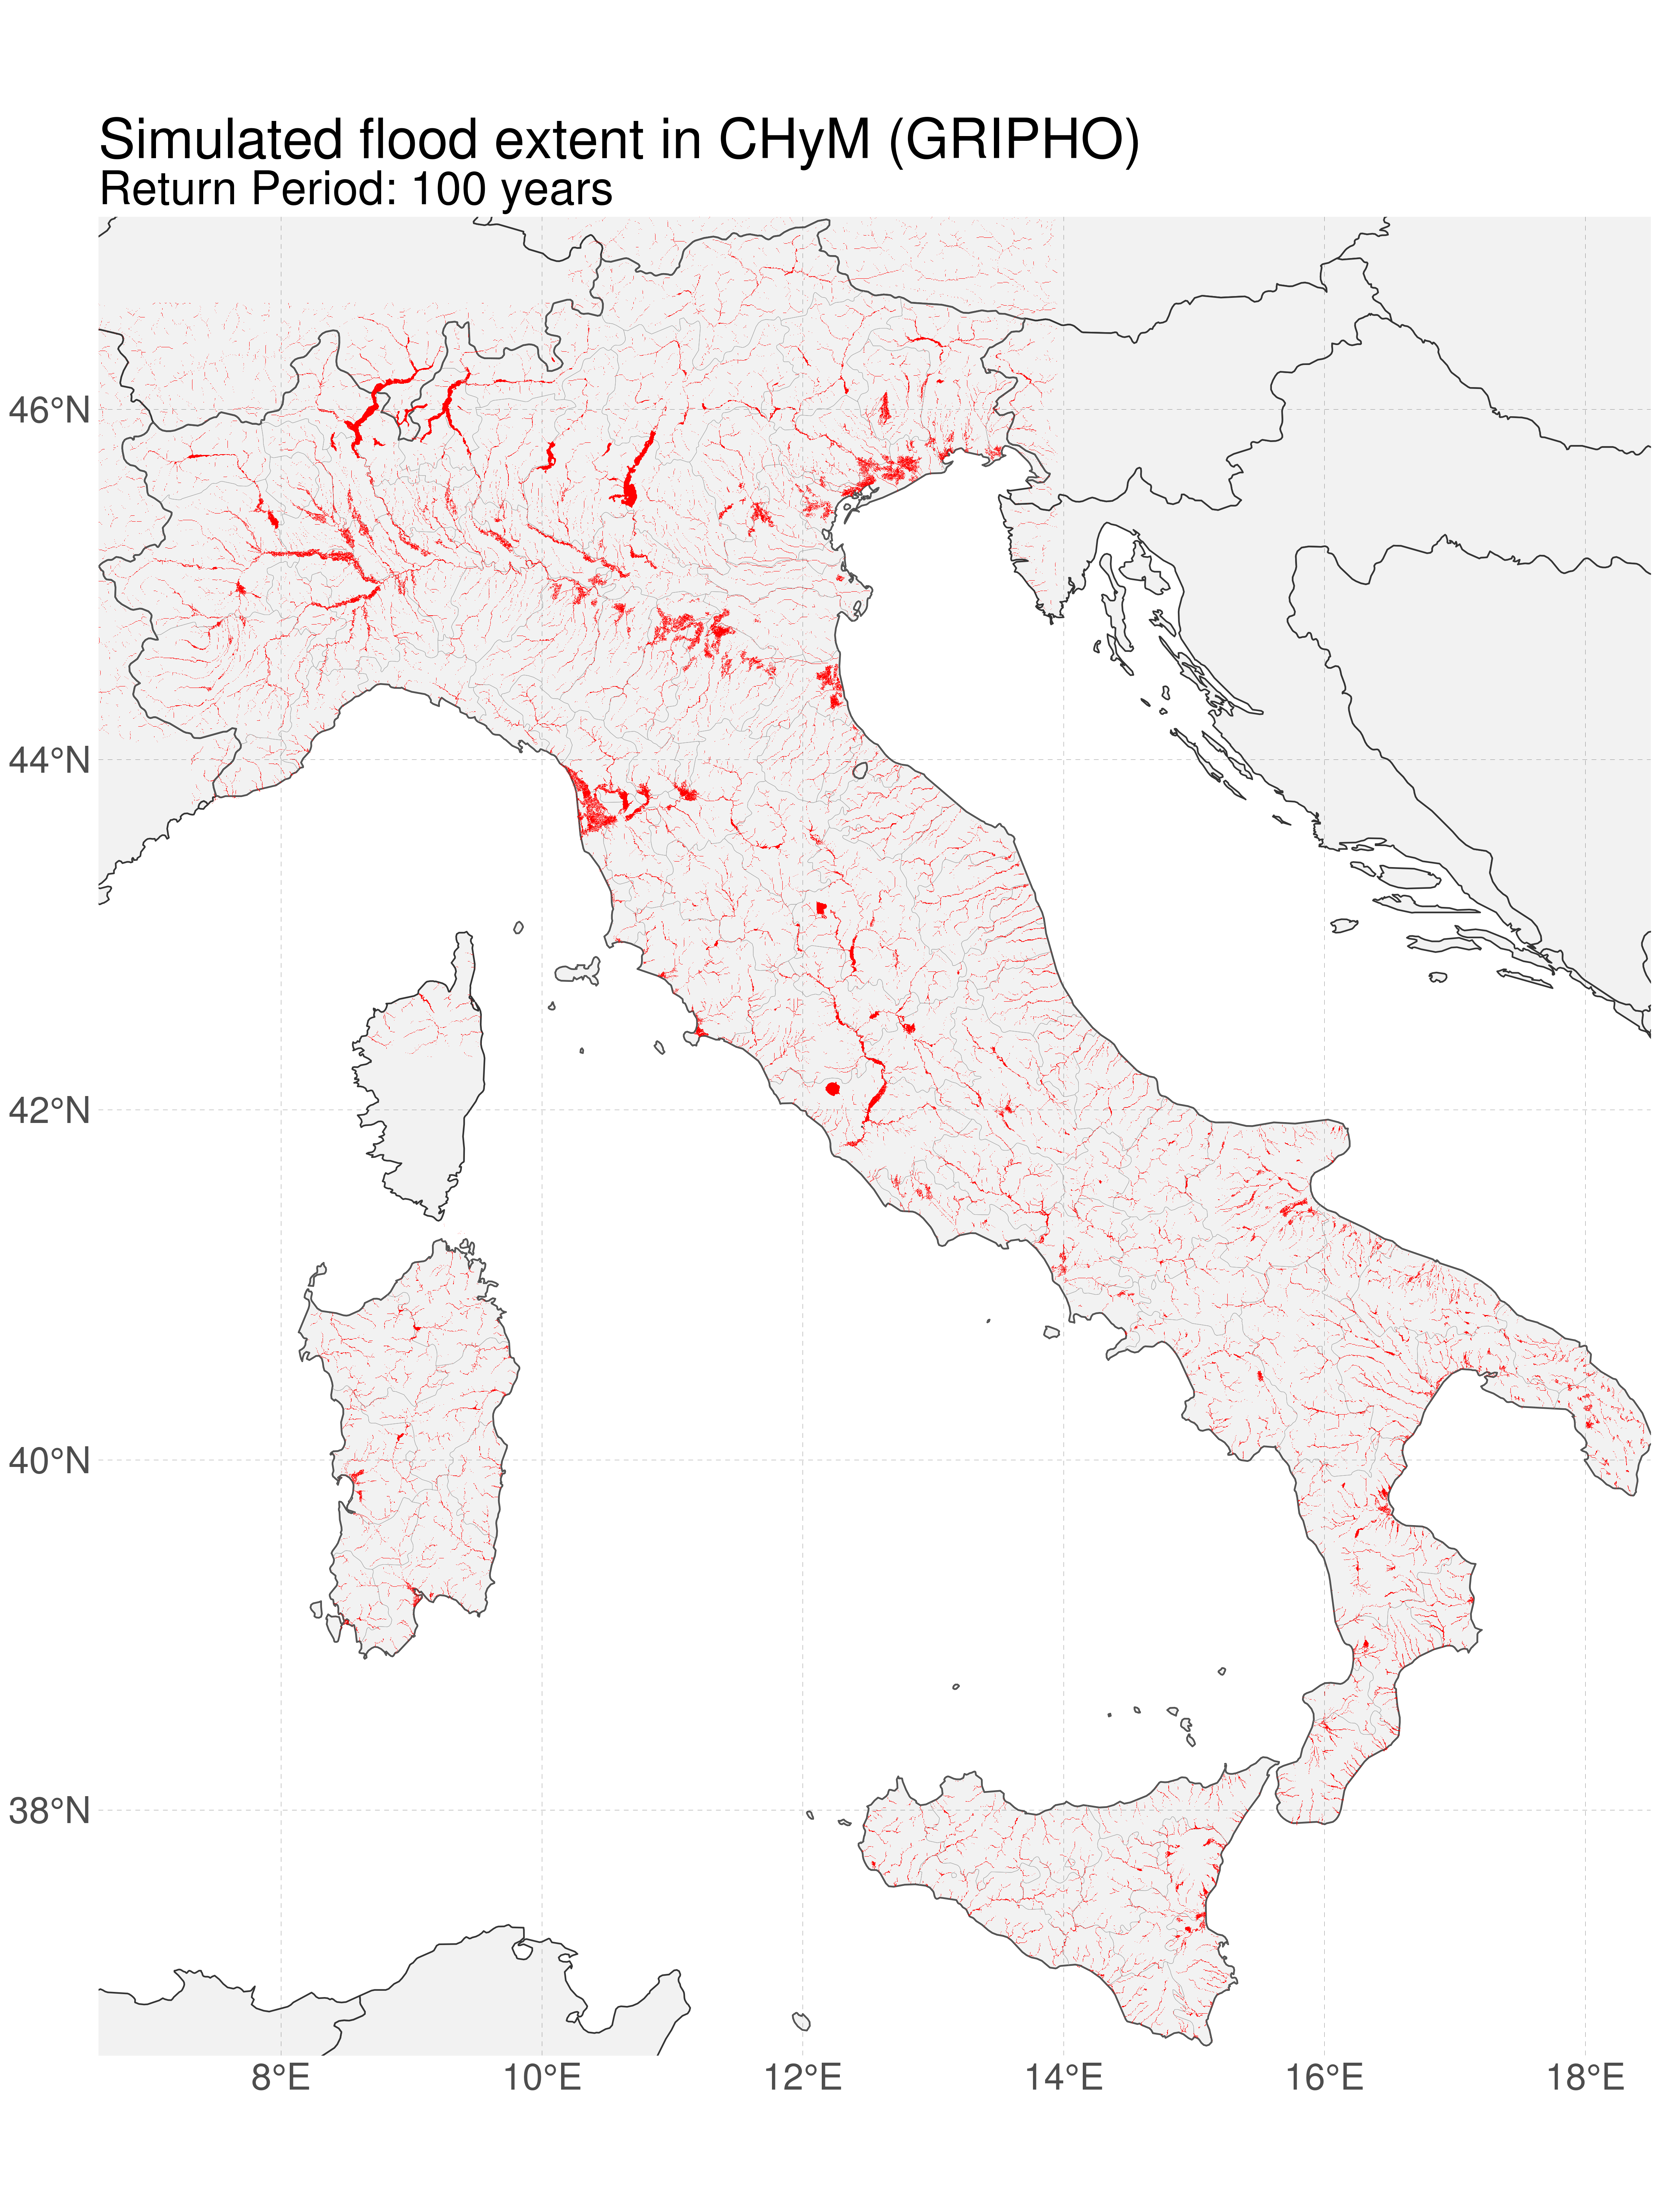
\includegraphics[width=\textwidth]{figures/valid_flood/flooded_areas/T100}
    \end{subfigure}\\
    \begin{subfigure}{.49\textwidth}
        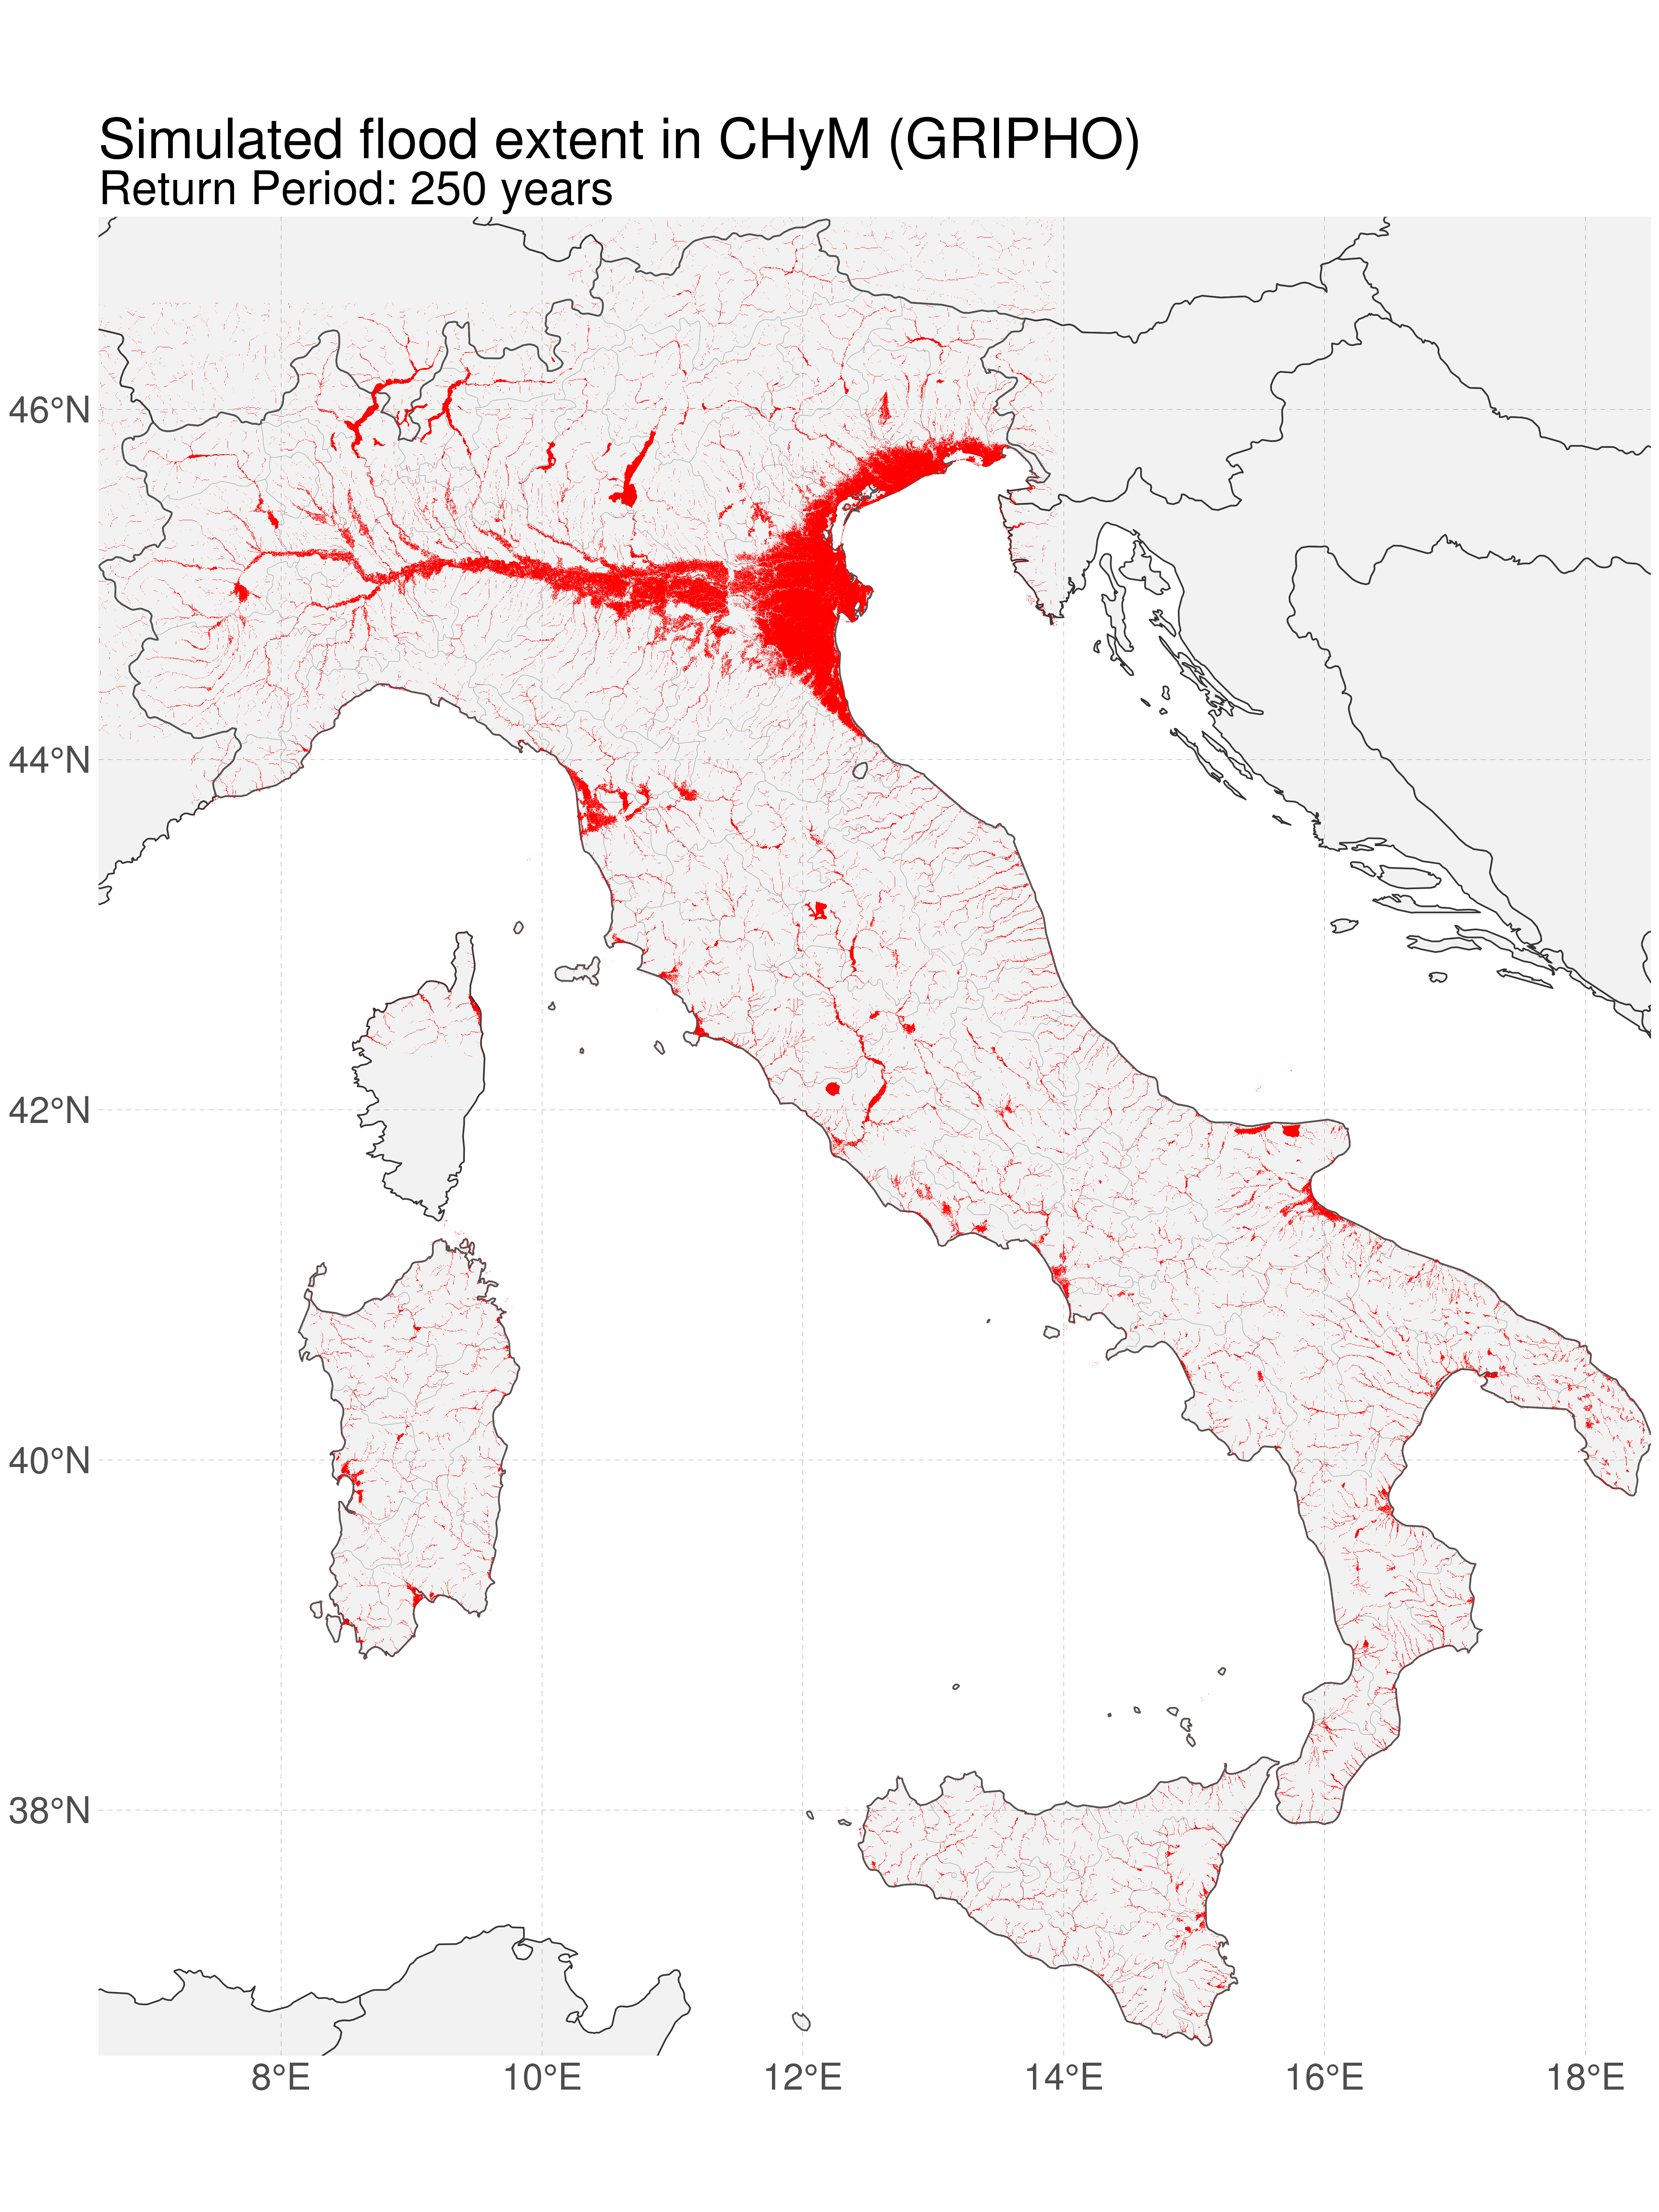
\includegraphics[width=\textwidth]{figures/valid_flood/flooded_areas/T250}
    \end{subfigure}
    \begin{subfigure}{.49\textwidth}
        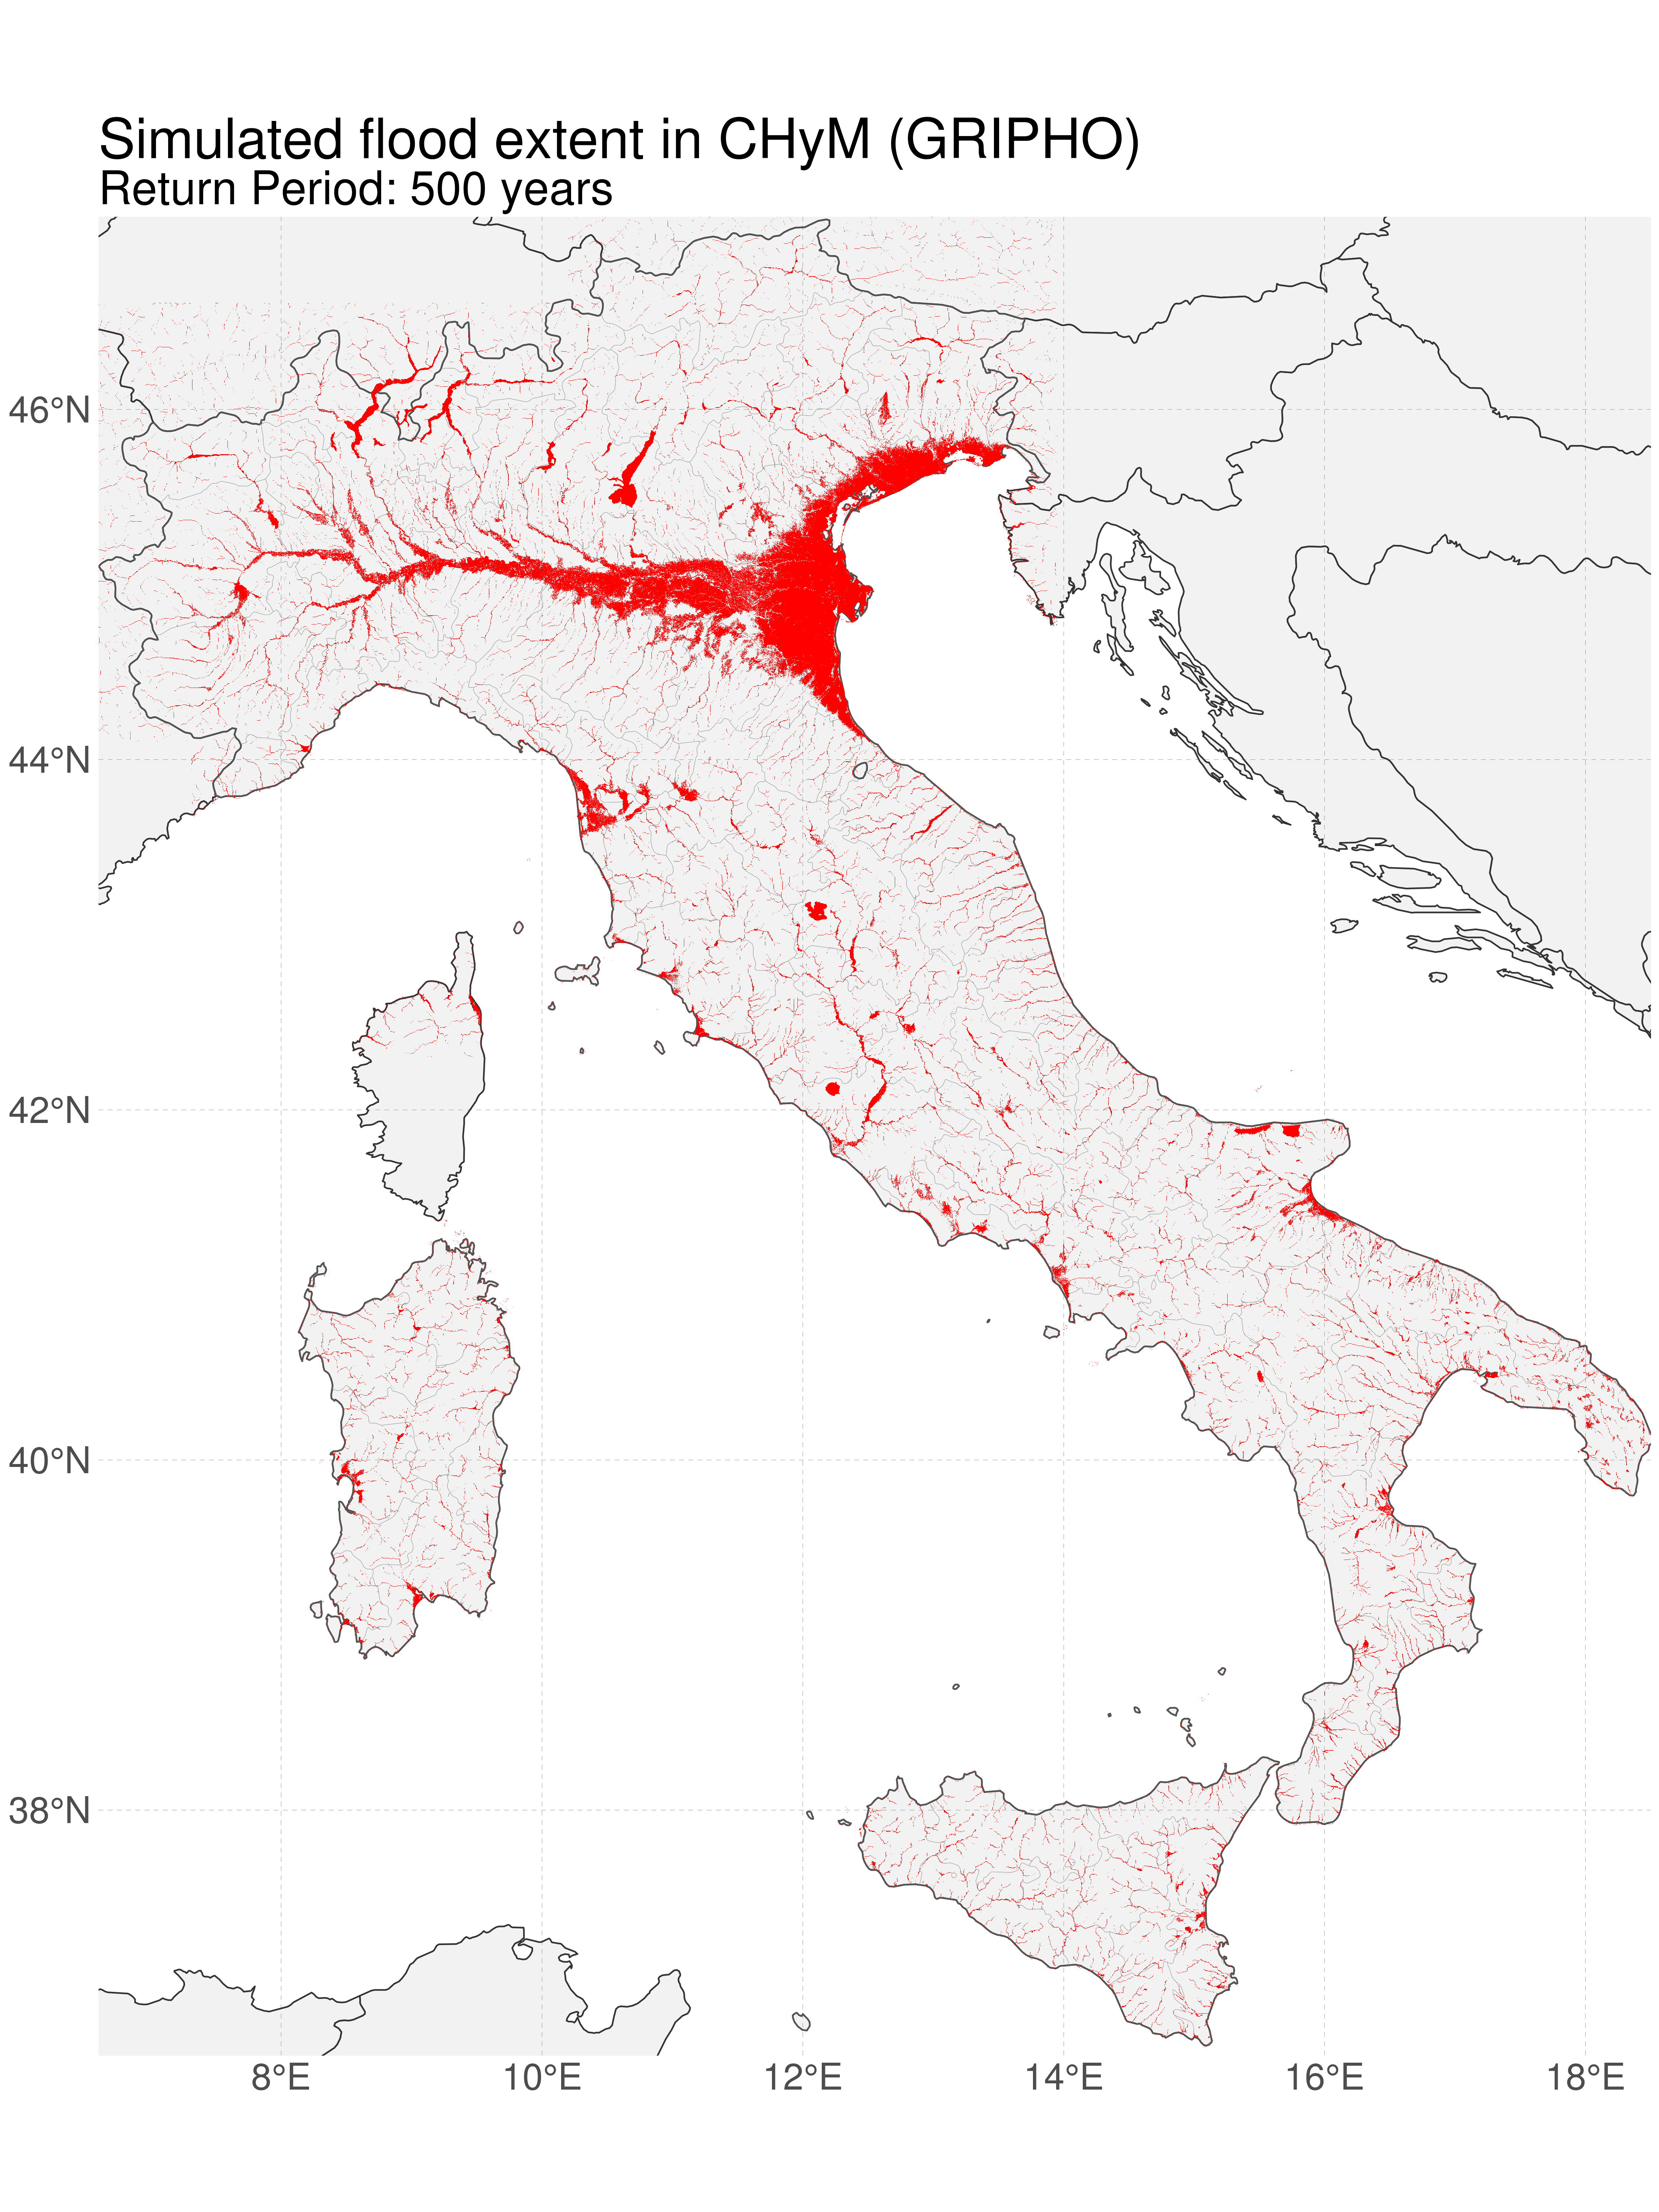
\includegraphics[width=\textwidth]{figures/valid_flood/flooded_areas/T500}
    \end{subfigure}
    \decoRule
    \caption[Flooded areas for RP = 50, 100, 250 and 500 years]{Preliminary results on the flooded area for four different Return Periods (50, 100, 250 and 500 years), computed by CA2D using data from an observation-driven CHyM simulation.} \label{fig:flooded_areas}
\end{figure}
